\documentclass[twocolumn]{svjour3}



\usepackage{francois-preamble}
%\usepackage[pdftex]{graphicx}
\usepackage{wrapfig}
%
%\usepackage{amsmath,amssymb}
\usepackage{bm}
\usepackage{algorithmic}
\usepackage{array}

%\graphicspath{{/home/francois/Dropbox/PaperHenrikMeSune/jmiv/figures/}}
\graphicspath{{figures/}}


% Frank Mittelbach's and David Carlisle's array.sty patches and improves
% the standard LaTeX2e array and tabular environments to provide better
% appearance and additional user controls. As the default LaTeX2e table
% generation code is lacking to the point of almost being broken with
% respect to the quality of the end results, all users are strongly
% advised to use an enhanced (at the very least that provided by array.sty)
% set of table tools. array.sty is already installed on most systems. The
% latest version and documentation can be obtained at:
% http://www.ctan.org/pkg/array


% IEEEtran contains the IEEEeqnarray family of commands that can be used to
% generate multiline equations as well as matrices, tables, etc., of high
% quality.




% *** SUBFIGURE PACKAGES ***
%ifCLASSOPTIONcompsoc
  %\usepackage[caption=false,font=normalsize,labelfont=sf,textfont=sf]{subfig}
\usepackage[caption=false,font=footnotesize,labelfont=sf,textfont=sf]{subfig}



\usepackage{url}

% correct bad hyphenation here
\hyphenation{op-tical net-works semi-conduc-tor}
\makeatletter
%\def\cl@chapter{\cl@chapter \@elt {theorem}}%bug in class
\def\cl@chapter{\@elt {theorem}}
\makeatother

\newcommand\red[1]{\color{red}#1}
\newcommand\violet[1]{\color{violet}#1}
\newcommand{\francois}[1]{{\color{red}\textbf{Francois: }#1}}
\newcommand{\Sune}[1]{{\color{green}\textbf{Sune: }#1}}



\usepackage{enumitem}
\usepackage{float}
\usepackage{cleveref}
\usepackage{todonotes}
\usepackage{tikz}
\usepackage{tikz-cd}


\author{Henrik G. Jensen \and Fran\c{c}ois Lauze \and Sune Darkner}
\institute{H. G. Jensen \at Dept. of Computer Science, University of Copenhagen \\
  \email{henrikgjensen@gmail.com}
  \and F. Lauze \at
  Dept. of Computer Science, University of Copenhagen \\
  \email{francois@di.ku.dk}           %  \\
  \and
  S. Darkner\at
  Dept. of Computer Science, University of Copenhagen \\
  \email{darkner@diku.dk}           %  \\
  }


\begin{document}

\title{Information-Theoretic Registration with Explicit Reorientation of Diffusion-Weighted Images}


% make the title area
\maketitle



\begin{abstract}
  We present an information-theoretic approach to registration of DWI with explicit
  optimization over the orientational scale, with an additional focus on normalized mutual
  information as a robust information-theoretic similarity measure for DWI. The framework
  is an extension of the LOR-DWI density-based hierarchical scale-space model, that varies
  and optimizes over the integration, spatial, directional, and intensity scales. We
  extend the model to non-rigid deformations and show that the formulation provides
  intrinsic regularization through the orientational information. Our experiments
  illustrate that the proposed model deforms ODFs correctly and is capable of handling the
  classic complex challenges in DWI-registrations, such as the registration of
  fiber-crossings along with kissing, fanning and interleaving fibers. Our results clearly
  illustrate a novel promising regularizing effect, that comes from the nonlinear
  orientation-based cost function. We illustrate the properties of the different image
  scales, and show that including orientational information in our model make the model
  better at retrieving deformations compared to standard scalar-based registration.
\end{abstract}

% Note that keywords are not normally used for peerreview papers.
% \begin{IEEEkeywords}
%   Registration, Diffusion-Weighted MRI, Normalized Mutual Information, Explicit
%   Reorientation, Analytical Gradients, Density-Based Formulation, Watson Density Function,
%   Free-Form Deformation, Cubic B-Spline.
% \end{IEEEkeywords}}




% To allow for easy dual compilation without having to reenter the
% abstract/keywords data, the \IEEEtitleabstractindextext text will
% not be used in maketitle, but will appear (i.e., to be "transported")
% here as \IEEEdisplaynontitleabstractindextext when the compsoc 
% or transmag modes are not selected <OR> if conference mode is selected 
% - because all conference papers position the abstract like regular
% papers do.
%\IEEEdisplaynontitleabstractindextext
% \IEEEdisplaynontitleabstractindextext has no effect when using
% compsoc or transmag under a non-conference mode.







% For peer review papers, you can put extra information on the cover
% page as needed:
% \ifCLASSOPTIONpeerreview
% \begin{center} \bfseries EDICS Category: 3-BBND \end{center}
% \fi
%
% For peerreview papers, this IEEEtran command inserts a page break and
% creates the second title. It will be ignored for other modes.
%\IEEEpeerreviewmaketitle



\section{Introduction}
\francois{Attempt to start more "generically":}
In this work, we study registration problems for images of the type $I:\Omega\to \Ff(\PP^2)$ with $\Omega$ an open, bounded domain of $\RR^3$, 
the image domain, $\PP^2$ is the projective plane of directions in $\RR^3$ and $\Ff(\PP^2)$ is a suitable function space on $\PP^2$: each $I(\bx)$ is a function  $I(\bx):\PP^2\to\RR$ which weights three-dimensional directions . We may and will also reinterpret such an image $I$ as an image $\bI:\Omega\times\PP^2\to\RR$, $\bI(\bx, \bs) = I(\bx)(\bs)$. These functions can be used to represent orientation distribution functions often used in Diffusion Weighted Imaging (DWI).
\francois{Could we use distrubutions on $\PP^2$ instead of functions? It would be closer to the classical ODFs? Need to check whether the rest of the text
would need adaptation or not.}

DWI is a non-invasive Magnetic Resonance Imaging (MRI) protocol that can
be used to infer microstructures of biological tissues by tracking the movement of water molecules, otherwise
invisible in structural MRI. However, the geometry of DWI makes it a challenge in image
registration, a key tool for comparing and analyzing medical image data. In addition, DWI
acquired on different scanners or with different protocols have a non-linear relationship
and defining the similarity between two DWI is inherently
difficult. \cite{johansen2013diffusion}.
%notably high-angular resolution diffusion imaging (HARDI) which models complex displacement profiles.


Our contribution is a scale-space formulation of density estimation for image similarity
for DWI in a nonrigid registration setting. The model encompasses explicit reorientation
providing the computational framework for estimating non-linear similarity measures
well-suited for DWI. The model allows for image similarities such as normalized mutual
information (NMI) by extending the Locally Orderless Registration for Diffusion-Weighted
Images (LOR-DWI) \cite{jensen2015locally} to nonrigid registration. LOR-DWI includes
orientational information in the image similarity, which allows explicit optimization over
the reorientation of diffusion gradients. This extends from DTI to the raw high-angular
resolution scans (HARDI) or the topographically inverted Orientation Density Functions
(ODF).

We demonstrate the properties of the framework, such as the effect of the reorientation on
the ODFs, the effect of the scale-space on optimization and regularization on simulated
DWI data and on a synthetic deformation of data from a subject of the Human Connectome
Project (HCP) \cite{van2013wu}. We show that LOR-DWI formulation preserves the ODFs and
produce excellent mappings for crossing, kissing and curving fibers, while providing an
inherent regularizing effect.


% The density formulation also allows us to optimize over the isocurves of the DWI signal,
% as the 5D image structures ($\mathbb{R}^3\times\mathbb{P}^2$) are defined in a joint
% histogram.


  %We extend the Locally Orderless Registration for Diffusion-Weighted Images (LOR-DWI)
  % \cite{jensen2015locally} framework to a nonrigid formulation. The LOR-DWI is a
  % scale-space framework for DWI density estimation that allows for a wide range of
  % linear and non-linear similarity measures. The formulation includes the orientational
  % information in the objective function, which results in an explicit optimization over
  % the reorientation of diffusion gradients. This includes the raw high-angular
  % resolution scans (HARDI) or the topographically inverted Orientation Density Functions
  % (ODF). The density formulation also allows us to optimize over the isocurves of the
  % DWI signal, as the 5D image structures ($\mathbb{R}^3\times\mathbb{P}^2$) are defined
  % in a joint histogram.

  % Our contribution is a scale-space formulation of density estimation for image
  % similarity for DWI in a nonrigid registration setting with explicit reorientation
  % providing the computational framework for estimating non-linear similarity measures
  % well-suited for DWI, such as normalized mutual information (NMI). We demonstrate the
  % properties of the framework, such as the effect of the reorientation on the ODF's, the
  % effect of the scale space on optimization and regularization on simulated DWI data and
  % on a synthetic deformation of data from a subject of the Human Connectome Project
  % (HCP) \cite{van2013wu}. We show that LOR-DWI formulation preserves the ODF's produce
  % excellent mappings for crossing, kissing and curving fibers, preserves the topology of
  % the domain while providing intuitive match and has a inherent regularizing effect .

The density formulation also allows us to optimize over the isocurves of the DWI signal
$I:\mathbb{R}^3\times\mathbb{P}^2\rightarrow\mathbb{R}$.  In principle, this framework
could be extended to other non-trivial geometry of other image modalities where
scale-space structures can be defined. In this work, we focus on DWI data where we use a
classical scale-space structure on this non-linear geometry.


\section{Related Work}

This work addresses two major challenges in voxel-based registration of DWI: The
reorientation of DWI in image registration, and the non-linear similarity between DWI.

% DWI registration

Image registration refers to a process that transforms data into a shared coordinate
system. For DWI, the common way to register two images is to use scalar-based methods on
quantitative measures, such as the fractional anisotropy (FA) or the mean diffusivity (MD)
\cite{o2017advances}. However, as such methods disregard most of the directional
information in DWI, methods have been developed to also account for the reorientation of
the diffusion profile. Most of these are created on top of scalar-based methods and
iteratively reorients the gradients after changing the deformation field. Some of the most
popular methods can be found in
\cite{avants2009advanced,tournier2012mrtrix,jenkinson2012fsl,
  fischl2012freesurfer}. However, registration frameworks have also been designed with an
objective function that explicitly optimizes over the reorientation of the gradients, such
as \texttt{DTI-TK} \cite{zhang2006deformable}, \texttt{DT-REFineD} \cite{yeo2009dt}, and
the more recent \texttt{DR-TAMAS} \cite{irfanoglu2016dr}. These frameworks have been shown
to generally outperform scalar-based frameworks for DWI
\cite{wang2011dti,zhang2014large,wang2016evaluation,wang2017evaluations}. %Calculating the analytical gradients required for explicit reorientation, and in a computationally feasible way.

% DWI similarity

For scalar based approaches to image similarity, registration is straightforward as any
popular scalar-based measure can be used, e.g. the sum-of-squares difference (SSD)
\cite{yeo2009dt} or mutual information (MI)
\cite{wells1996mmv,wang2017evaluations}. Explicit reorientation strategies inherently
define the similarity over both position and orientation and, once the full diffusion
profile is part of the similarity, such measures can be defined in a well-suited way for
the non-linear relationship between DWI. Both \cite{zhang2006deformable} and
\cite{yeo2009dt} used variations on SSD in the objective function, while MI was used in
\cite{jensen2015locally} through an extension of the LOR framework in
\cite{darkner2013locally}. As argued in \cite{jensen2015locally}, the invariant and
statistical properties of MI makes it a logical choice for DWI, where multiple factors
result in a more statistical relationship, such as variations in $b$-values,
non-monoexponential behavior in biological tissue, and inter-scanner variability
\cite{johansen2013diffusion}. MI is often used in the standard registration of complex
modalities and, as such, in scalar-based registration of DWI \cite{van2007nonrigid} and in
the pre-processing of DWI \cite{treiber2016characterization}. MI and normalized MI (NMI)
\cite{studholme1999overlap} provides a non-linear statistical measure for DWI. However, it
is also likely that more functional measures could be well-suited, such as
cross-correlation (CC) and normalized CC (NCC), both of which can be defined from the LOR
density-formulation \cite{sporring2011jacobians,darknersporring2012pami}. The
density-based DWI comes from the generalized way of estimating image similarity measures
based on Locally Orderless Images (LOI) \cite{koenderink1999structure}. The first mention
of LOI in the context of image registration was in \cite{hermosillo2002variational} where
a variational approach to image registration was presented. The LOR framework
\cite{darknersporring2011ipmi,darknersporring2012pami} generalized a range of similarity
measures as linear and non-linear functions of density estimates for scalar-valued images.


\section{Locally Orderless DWI}
\label{sec:lor_dwi}
\subsection{Notations}
We start by introducing a few necessary notations. $\Omega\subset \mathbb R^3$ is the
spatial domain of the images under consideration. A scalar image is a function
$\bm I:\Omega\to\mathbb R^3$. We assume that we can extend it on the whole $\mathbb R^3$,
for instance by extending it with 0. The projective space of directions of $\mathbb R^3$
is denoted by $\mathbb P^2$, and the unit sphere of $\mathbb R^3$ by $\mathbb S^2$.  We
will encounter \emph{spatio-directional} images
$\bm I:\Omega\times \mathbb P^2 \to \mathbb R$, which we similarly assume too be
extendable to $\mathbb R^3\times \mathbb P^2$. This is necessary in both cases in order to
define their spatial smoothing via convolution. We use the following elementary property:
As $\mathbb P^2$ can naturally be identified as the quotient $\mathbb S^2/\{\pm 1\}$ by
the antipodal symmetry, a function $f:\mathbb P^2\to \mathbb R$ can be lifted to an
antipodal symmetric function $\tilde{f}:\mathbb{S}^2\to \mathbb{R}$. Conversely, any
antipodal symmetric function $g:\mathbb S^2\to \mathbb R$ factors through $\mathbb P^2$.
A spatio-directional image can (and will) be lifted to an antipodal symmetric image
$\tilde{\bm I}:\Omega\times \mathbb S^2$:
$\tilde{\bm I}(\bm x, -\bm v) =\tilde{\bm I}(\bm x, \bm v)$.  We will denote by $\bm I$
both the spatio-directional image and its antipodal symmetric lifting in the following.

\subsection{Recall on the LOR Framework}
The LOR framework defines the density estimates over three scales: The image scale
$\sigma$, the intensity scale $\beta$, and the integration scale $\alpha$. In the context
of scalar registration, for a transformation $\phi:\mathbb{R}^3\rightarrow\mathbb{R}^3$,
the estimated histogram $h$ and the corresponding density $p$ is computed as
\begin{align}
\label{eq:loih}
  h_{\beta\alpha\sigma}&(i,j|\phi,\bm x)=\\
                 &\int_{\mathbb R^3}P_\beta( \bm I_{\sigma}(\phi(\bm x))-i)
                   P_\beta( \bm J_{\sigma}(\bm x)-j)W_\alpha(\bm \tau-\bm x)d\bm \tau\nonumber \\
  \label{eq:loipdf}
  p_{\beta\alpha\sigma}&(i,j|\phi,\bm x)\simeq \frac{h_{\beta\alpha\sigma}(i,j|\phi,\bm x)}
                         {\int_{\Lambda^2} h_{\beta\alpha\sigma}(k,l|\phi,\bm x)dk\; dl}
\end{align} 
where $i,j\in[a_1, a_2] =: \Lambda$ are values in the image intensity range,
$\bm I_{\sigma}(\bm \phi(\bm x))=(\bm I*K_\sigma)(\bm \phi(\bm x))$ and
$ J_{\sigma}(\bm x)=(\bm J*K_\sigma)(\bm x)$ are images convolved with the kernel
$K_\sigma$ with standard deviation $\sigma$, $P_\beta$ is a Parzen-window of scale
$\beta$, and $W_\alpha$ is a Gaussian integration window of scale $\alpha$. The marginals
are trivially obtained by integration over the appropriate variable.  The LOR-approach to
similarity lets us use a set of generalized similarity measures, the linear and non-linear
\begin{align}\label{eq:sim}
  \mathcal{F}_{lin}=\int_{\Lambda^2}f(i,j)p(i,j)di\; dj\\ \mathcal{F}_{non-lin}=\int_{\Lambda^2}f(p(i,j))di\; dj
\end{align}
where the linear measure $f(i,j)$ includes e.g. sum of squared differences and Huber, and
the non-linear $f(p(i,j))$ includes e.g. MI, normalized MI (NMI), see
\cite{darknersporring2012pami} for details.

\subsection{The LOR-DWI framework}

This work addresses the estimation of the image similarity $\mathcal F$ of DWI in the
context of nonrigid registration an extension of our previous work
\cite{jensen2015locally}.
In this context, $\bm I$ and $\bm J$ are spatio-directional signals. Specifically, DWI MR
attenuation signals at location $\bm x$, for a gradient direction $\bm v$, are modeled by
$S(\bm x,\bm v) = S_0(\bm x) e^{-b\bm I(\bm x,\bm v)}$ \ \cite{tao2006method} and apparent
diffusion coefficients volumes are given by
$\bm I(\bm x,\bm v)=-\frac{1}{b}\log\frac{S(\bm x,\bm v)}{S_0(\bm x)}$. Gradient
directions $\bm v$ belong to $\mathbb S^2$ but the diffusion is orientation-free such that
$\bm I(\bm x,\bm v)\approx \bm I(\bm x,-\bm v)$ which naturally defines a
spatio-directional image $\Omega\times \mathbb P^2 \to \mathbb R$.  In order to apply
LOR-DWI, the histogram and density estimates \Cref{eq:loih} and \cref{eq:loipdf} must be
extended to spatio-directional data, and the action of the spatial transformation on the
directions must be defined.

We introduce a kernel on the sphere as an extension to the density estimates of LOR to
include directional information. This kernel accounts for directional smoothing and
defines our LOR-DWI framework.  Thus, we extend spatial smoothing to be
spatio-directional, such that the directional smoothing preserves this symmetry and the
projective structure, via a symmetric kernel $\Gamma_\kappa(\bm \nu,\bm v)$ on
$\mathbb{S}^2$. We define the smoothed signal $\bm I_{\sigma,\kappa}$ at scales
$(\sigma,\kappa)$ by
\begin{align}
  \bm I_{\sigma\kappa}(\bm x,\bm v)&=\label{eq:vecfieldsmooth}
      \int_{S^2} \left( \int_{\mathbb R^3} \bm I(\bm \tau,\bm \nu)K_\sigma(\bm \tau-\bm x)d\bm \tau\right) 
     \Gamma_{\kappa}(\bm \nu, \bm v) d\bm \nu\nonumber\\&=(\bm I*(K_{\sigma}\otimes \Gamma_{\kappa}))(\bm x,\bm v)
\end{align}
where $K_\sigma(\bm x)$ is a Gaussian kernel with $\sigma$ standard deviation.  We employ
a symmetric Watson distribution \cite{jupp1989unified} as $\Gamma_{\kappa}(\bm \nu,\bm v)$
for directional smoothing on $\mathbb S^2$, given by
\begin{align}
&\Gamma_\kappa(\bm \nu,\bm v)=Ce^{\kappa({\bm \nu}^\top \bm v)^2}\\ &C=M(\frac{1}{2},\frac{1}{d},\kappa)
\end{align}
where $M(\frac12,\frac{d}2,\kappa)$ the confluent hypergeometric function also called the
Kummer function ($d=3$ in our case) \cite{AbramowitzStegun1974}, $\pm\bm v$ the center of
the distribution, and $\kappa$ the concentration parameter, which is roughly inverse
proportional to the variance on the sphere. Because of the symmetry property of the Watson
distribution and the antipodal symmetry of $\bm I(\bm x,\bm v)$, it is clear that
$\bm I_{\sigma\kappa}(\bm x,\bm v)$ is antipodal symmetric too. As one alternative, a
symmetrized von Mises-Fisher \cite{jupp1989unified} distribution or a symmetrized heat
kernel could be considered.

\subsubsection{Action on Orientation}
A transformation $\phi:\Omega\to \Omega$ acts on directions via its Jacobian: at
${\bm x}\in \Omega$, $J_x\phi$ sends $\mathbb R\bm v$ to $\mathbb R J_{\bm x}\phi \bm v$
which is well-defined as soon as $\det(J_{\bm x}\phi)\not = 0$ which is the case if we
assume that $\phi$ is diffeomorphic. Via the representation
$\mathbb{P}^2\simeq \mathbb{S}^2/\{\pm1\}$, we can write
$\mathbb P_{\bm x}\phi:\{\pm v\} \mapsto \{\pm\frac{J_{\bm x}\bm v}{|J_{\bm x}\bm v|}\}$.
We denote by $\psi$ the mapping
$(\bm x,\bm v)\mapsto \frac{J_{\bm x}\bm v}{|J_{\bm x}\bm v|}$. Because it will only
appear inside an antipodal symmetric kernel, $\psi_{\bm x} = \psi(\bm x,\cdot)$ represents
$\mathbb P_{\bm x}\phi$ \emph{without ambiguity}. Because of spatial convolutions, we
assume that $\phi$ can be extented to $\mathbb R^3$, assuming that it is the identity out
of a compact set $D$ containing $\Omega$.

\subsubsection{Density, orientation and transformation}
In the following, we will often omit the parameter $\bm x$. We set $\Phi = (\phi,\psi)$,
and we write the joint histogram and density for similarity in image registration as
\begin{align}
  h_{\beta\alpha\sigma\kappa}&(i,j|\Phi,\bm x)=\\ 
                      &\int_{\mathbb R^3 \times S^2}P_\beta(\bm I_{\sigma\kappa}(\phi(\bm x),\psi(\bm v))-i)
                        P_\beta(\bm J_{\sigma\kappa}(\bm x,\bm v)-j)\nonumber \\
                      &W_\alpha(\bm \tau-\bm x)d\bm \tau\times d\bm v \nonumber \label{eq:densityreg} \\
                      &p_{\beta\alpha\sigma\kappa}(i,j|\Phi,\bm x)=\frac{h_{\beta\alpha\sigma\kappa}(i,j|\Phi,\bm x)}
                       {\int_{\Lambda^{2}} h_{\beta\alpha\sigma\kappa}(i,j| \Phi,\bm x)dl\;dk} \;\;.
\end{align}
Assume that $W$ is a Gaussian kernel with standard deviation $\alpha$. If we left
$\alpha\rightarrow\infty$, we would obtain full spatial integration and can ignore the
integration scale $\alpha$.

\subsection{LOR-DWI and Free Form Deformation}
In \cite{jensen2015locally}, we assumed that $\phi$ was a global affine transformation,
with $\psi_x = \psi$ being the projectivization of its linear part. In the present work,
we assume $\phi$ to be a nonrigid transformation, and we use Rueckert \textit{et al.\/}
framework \cite{rueckert1999nonrigid} where the transformation $\phi$ is given as a
hierarchical spline representation \emph{linearly} parameterized by a spatial grid of
control points ${\bm c}$. In the next subsection, we use its vectorized form, so that
$\phi = \bm B\bm c$, $\Phi_{\bm c} = (\phi_{\bm c},\psi_{\bm c})$. We seek the
transformation $\Phi^*_{\bm c}$ which maximizes the regularized NMI
\begin{align}
  \Phi_c^* = \operatorname*{arg\,max}_c \mathcal M(\Phi_c) = \operatorname*{arg\,max}_c \mathcal F(\bm I\circ\Phi_c,\bm J)+\mathcal S({\Phi_c})
    \label{eq:argmax}
\end{align}
The dependency of $\mathcal M$ in $\bm c$ is complex. The following dependency diagram
(Fig. \ref{fig:dependcygraph}) for the mutual information term illustrates it.
\begin{figure}[ht]

\begin{equation*}
\begin{tikzcd}[column sep=0.4cm,row sep=0.5cm]
  ~& NMI( \bm I_{\sigma\kappa}\circ\Phi_{\bm c},\bm J_{\sigma\kappa};\beta)&~\\
  H_{\bm I_{\sigma\kappa}\circ\Phi_{\bm c};\beta} \ar[ur]&  
  H_{\bm J_{\sigma\kappa};\beta}\ar[u] & 
  H_{\bm I_{\sigma\kappa}\circ\Phi_{\bm c}, \bm J_{\sigma\kappa};\beta}\ar[lu]\\
  p_{\beta,\bm I_{\sigma\kappa}\circ\Phi_{\bm c}}\ar[u]  & 
  p_{\beta,\bm J_{\sigma\kappa}}\ar[u]  & 
  p_{\beta,\bm I_{\sigma\kappa}\circ\Phi_{\bm c}, \bm J_{\sigma\kappa}}\ar[u]\\
  ~ & h_{\beta,\bm I_{\sigma\kappa}\circ\Phi_{\bm c},\bm J_{\sigma\kappa}}\ar[ul]\ar[u]\ar[ur]& ~\\
  \bm I_{\sigma\kappa}(\phi_{\bm c},\psi_{\bm c})\ar[ur]&\psi_{\bm c}\ar[l]&\bm J_{\sigma\kappa}\ar[ul]\\
  \boxed{\bm c}\ar[r ]& \phi_{\bm c}\ar[lu] \ar[u]&
  \ar[from=1-1,to=1-3,color=red,dash,line width=0.65pt,start
  anchor={[xshift=-2.2em,yshift=2ex]center},end
  anchor={[xshift=+3.1em,yshift=2ex]center}]
  % 
  \ar[from=1-1,to=4-1,color=red,dash,line width=0.65pt,start
  anchor={[xshift=-2.2em,yshift=2ex]center},end
  anchor={[xshift=-2.2em,yshift=-1.5ex]center}]
  %
  \ar[from=4-1,to=4-3,color=red,dash,line width=0.65pt,start
  anchor={[xshift=-2.2em,yshift=-1.5ex]center},end
  anchor={[xshift=+3.1em,yshift=-1.5ex]center}]
  %
  \ar[from=1-3,to=4-3,color=red,dash,line width=0.65pt,start
  anchor={[xshift=+3.1em,yshift=2ex]center},end
  anchor={[xshift=+3.1em,yshift=-1.5ex]center}]
  %
  \ar[from=5-1,to=5-2,color=blue,dash,line width=0.65pt,start
  anchor={[xshift=-2.6em,yshift=1.7ex]center},end
  anchor={[xshift=+0.9em,yshift=1.7ex]center}]
  %
  \ar[from=6-1,to=6-2,color=blue,dash,line width=0.65pt,start
  anchor={[xshift=-2.6em,yshift=-1.7ex]center},end
  anchor={[xshift=+0.9em,yshift=-1.7ex]center}]
  %
  \ar[from=5-1,to=6-1,color=blue,dash,line width=0.65pt,start
  anchor={[xshift=-2.6em,yshift=1.7ex]center},end
  anchor={[xshift=-2.6em,yshift=-1.7ex]center}]
  %
  \ar[from=5-2,to=6-2,color=blue,dash,line width=0.65pt,start
  anchor={[xshift=+0.9em,yshift=1.7ex]center},end
  anchor={[xshift=+0.9em,yshift=-1.7ex]center}]
\end{tikzcd}
\end{equation*}
\caption{Dependency graph of the nonrigid DWI registration between the moving image
  $\bm I$ and the target image $\bm J$, with normalized mutual information (NMI) as the
  similarity measure. The deformation is parameterized by $\bm c$ so that any change in
  $\bm c$ will eventually affect the total similarity between the two images. The red
  frame contains MI registration elements which are classical, while the blue frame
  contains the part which extends the LOR framework to the LOR-DWI.}
    \label{fig:dependcygraph}
\end{figure}

\subsection{Estimation and optimization of similarity} 
We use quasi-Newton methods to compute an optimum of \Cref{eq:argmax}, in particular
L-BFGS\cite{} from \cite{schmidt2005minfunc}, and thus need to compute the gradient of the
similarity with respect to control points vector $\bm c$. Most of the required
calculations are provided in
\cite{rueckert1999nonrigid,darknersporring2012pami,jensen2015locally}, they correspond to
the red frame in Figure \ref{fig:dependcygraph}, a full formula for the gradient is long
and not informative for the present work. We therefore only describe how
spatio-directional smoothing contributes to the image similarity, i.e., the part of Figure
\ref{fig:dependcygraph} enclosed in the blue frame. Thanks to the LOR-DWI representation,
the present extension only appears within the spatio-directional smoothing of $\bm I$.
One complication originates from choices in our implementation, where the Kummer function
$M(\frac12, \frac32, \kappa)$ as the normalization constant in the Watson kernel is
replaced by an estimate of this factor from a discrete set of $N$ directions
$\nu_1,\dots,\nu_N$ at each voxel $\bm x$. It can therefore no longer be considered
constant. We rewrite the discrete spatio-directional smoothing as
\begin{align}
    {\bm I}_{\sigma \kappa}&(\phi_{\bm c}(\bm x), \psi_{\bm c}(\bm v)) =\nonumber\\
    &\sum_{n=1}^N \int_{\mathbb R^3}\bm I(\tau, \nu_n)K_\sigma(\phi_{\bm c}(\bm x)-\tau)
    \bar{\Gamma}_{\kappa}(\nu_n, \psi_{\bm c}(\bm v))\,d\tau
\end{align}
where we have set
\begin{equation}
 \label{eq:discreteWatson}
 \bar{\Gamma}_{\kappa}(\nu_n,\psi_{\bm c}(\bm v) =  \frac{e^{\kappa(\nu_n^\top\psi_{\bm c}(\bm v))^2}}
 {\sum_{i=1}^Ne^{\kappa(\nu_i^\top\psi_{\bm c}(\bm v))^2}} \;\; .
\end{equation}
We compute the Jacobian of the spatio-directional smoothing with respect to the control
point parameter $\bm c$:
\begin{align}
    J_{\bm c}{\bm I}_{\sigma \kappa}&(\phi_{\bm c}(\bm x), \psi_{\bm c}(\bm v)) =\nonumber\\
    &\sum_{n=1}^N\left(\int_{\mathbb R^3} \bm I(\tau, \nu_n)J_{\bm c}K_{\sigma}
    (\phi_{\bm c}(\bm x)-\tau)\,d\tau\right)\bar{\Gamma}_{\kappa}(\nu_n,\psi_{\bm c}(\bm v)  + \nonumber\\
    &\sum_{n=1}^N\left(\int_{\mathbb R^3} \bm I(\tau, \nu_n)K_{\sigma}
    (\phi_{\bm c}(\bm x)-\tau)\,d\tau\right)J_{\bm c}\bar{\Gamma}_{\kappa}(\nu_n,\psi_{\bm c}(\bm v) 
    \label{eq:sddirs}
\end{align}
From \cref{eq:sddirs}, we have
 \begin{align}
   J_{\bm c}K_\sigma(\phi_{\bm c}(\bm x)-\tau) = -\frac{K_\sigma(\bm\phi_{\bm c}(\bm x) - \tau)}{\sigma^2}
   \left(\phi_{\bm c}(\bm x)-\tau\right)^\top \bm B
 \end{align}
 because $K_\sigma$ is a Gaussian kernel with variance $\sigma^2$ and
 $\phi_{\bm c} = {\bm B}\bm c$, its Jacobian $J_{\bm c}\phi_{\bm c}$ is simply $\bm
 B$. The part involving directional kernel is somewhat more complex, as it involves the
 Jacobian $J_{\bm x}\phi_{\bm c}$ and the normalizing factor in \Cref{eq:discreteWatson}.
 Set $f(x) = e^{\kappa x^2}$ and define $f_i = f(\nu_i\top \psi_{\bm_c}(\bm v))$. Since
 $f'(x) = 2\kappa x f(x)$, we have
\begin{equation}
  J_{\bm c} f(\nu^\top\psi_{\bm c}\bm v) = 2\kappa
  f(\nu^\top\psi_{\bm c}(\bm v))\psi_{\bm c}(\bm v)^\top \nu\nu^\top J_{\bm c}\psi_{\bm c}(\bm v) \;\; .
\end{equation}
By a careful but straightforward calculation, we obtain
\begin{align}
    ~&J_{\bm c}\bar{\Gamma}_{\kappa}(\nu_n,\psi_{\bm c}(\bm v))=\\
    &-2\frac{\kappa\bar{\Gamma}_{\kappa}(\nu_n,\psi_{\bm c}(\bm v))}{\sum_{i=1}^N f_i}
    \psi_{\bm c}(\bm v)^\top\!\!\left(\sum_{i\not=n}\! f_i\nu_i\nu_i^\top\!\right)\!J_{\bm c}\psi_{\bm c}(\bm v)
\end{align}
To understand $J_{\bm c}\psi_{\bm_c}$, we need to deal with \emph{tensors}.  The matrix
$\bm B$ is built of cubic B-splines. With $k$ control points, $\bm c$ has dimension $3k$
and $\bm B(\bm x)\in \mathbb R^{3\times 3k}$. Its spatial Jacobian is a 3D-\emph{tensor}
made of quadratic B-splines, $J_{\bm x}\bm B\in \mathbb R^{3\times 3k\times 3}$.
$J_{\bm x}\phi_{\bm c} = J_{\bm x}\bm B\cdot \bm c$ where the '$\cdot$' operator
represents the \emph{contraction}
$\mathbb R^{3\times 3k\times 3}\times \mathbb R^{3k}\to \mathbb R^{3\times 3}$,
$(r_{uvw},s_{v})\mapsto \left(\sum_v r_{uvw} s_v\right)_{uw}$. One has
$ J_{\bm c}J_{\bm x}\phi_{\bm c} \in \mathbb R^{3\times 3\times 3k}\not= J_{\bm x}J_{\bm
  c}(\bm B\bm c) = J_{\bm x}\bm B\in \mathbb R^{3\times 3k\times 3}$, though the
difference is a matter of swapping indices.  $J_{\bm c}\psi_{\bm_c}$ is a 3D tensor of the
same order as $J_{\bm c}J_{\bm x}\phi_{\bm c}$. Another contraction comes from
$J_{\bm c}J_{\bm x}\phi_{\bm_c}(\bm v)$. This is a matrix in $\mathbb R^{3\times 3k}$ and
one can write $J_{\bm c}J_{\bm x}\phi_{\bm_c}(\bm v) = J_{\bm x}\bm B\bullet \bm v$ where
$\bullet$ is the contraction
$\mathbb R^{3\times 3k\times 3}\times \mathbb R^3 \to \mathbb R^{3\times 3k}$,
$(r_{uvw},t_w)\mapsto \left(\sum_{w} r_{uvw}t_w\right)_{uv}$.  The differentiation of the
inner product $\langle J_{\bm x}\phi_{\bm c}\bm v,J_{\bm x}\phi_{\bm c}\bm v\rangle$ is
given by
\begin{equation}
    J_{\bm c}\langle J_{\bm x}\phi_{\bm c}\bm v,J_{\bm x}\phi_{\bm c}\bm v\rangle = \left(J_{\bm x}\phi_{\bm c} \bm v\right)^\top \left(J_{\bm x}\bm B\bullet \bm v\right)
\end{equation}
Denoting by $\bm V$ the vector $J_{\bm x}\phi_{\bm c} \bm v$, so that $\psi_{\bm c}(\bm v) = \frac{\bm V}{|\bm V|}$,  the Jacobian $J_{\bm c}\psi_{\bm_c}\bm v$ is
\begin{equation}
    J_{\bm c}\psi_{\bm_c}\bm v = \left({\bf I}_3 - \frac{\bm V\bm V^\top}{|\bm V|^2}\right)\frac{J_{\bm x}\bm B\bullet \bm v}{|\bm V|}
\end{equation}
where ${\bf I}_3$ is the identity of $\mathbb R^3$. Note also that $\bm V = J_{\bm x}\phi_{\bm c} \bm v = \left(J_{\bm x}\bm B\cdot c\right)\bm v$ and that 
${\bf I}_3 - \frac{\bm V\bm V^\top}{|\bm V|^2}$ is the orthogonal projection ${\bm \pi}_{\bm V^\bot}$ onto $\bm V^\bot$, the plane orthogonal to $\bm V$.  
Putting things together, the Jacobian with respect to the control point parameter $\bm c$ of the spatio-directional smoothing is given by
\begin{align}
   \! \!\!~&J_{\bm c}{\bm I}_{\sigma \kappa}(\phi_{\bm c}(\bm x), \psi_{\bm c}(\bm v)) =\nonumber\\
    &\!\!-\sum_{n=1}^N\int_{\mathbb R^3} \bm I(\tau, \nu_n)K_\sigma(\phi_{c}(\bm x)-\tau)\bar{\Gamma}_\kappa(\nu_n,\psi_{\bm c}(\bm v))\times\nonumber\\
   &\!\!\left\{\!\! \frac{(\phi_{\bm c}(\bm x)-\tau)\!^\top\!\!\bm B}{\sigma^2}\!+\!\!\frac{2\kappa \bm V^\top\!\!\left(\sum_{i\not=n}\nu_i\nu_i^\top\!\right)}{|\bm V|\sum_{i=1}^N f_i}
  {\bm \pi}\!_{\bm V\!^\bot}\!\!\left(\frac{J_{\bm x}\bm B\bullet \bm v}{|\bm V|}\right)  
  \!\! \right\}\!d\tau.
\end{align}


\subsection{Regularization}
% Francois: reformulated from Henrik's paragraph.
So far, we have not specified the form of the regularizer $\mathcal S(\Phi_{\bm c})$ in
\Cref{eq:argmax}.  The regularization has received little attention due to the inherent
regularization from the smooth kernels and the additional directional structure. However,
we found that the last steps in the hierarchical transformation model required some
regularization to keep the deformation stable, due to the high resolution of the
deformation field. We used a simple regularization that penalizes a non-uniform grid by
the squared difference between a point $\bm c_i$ and its direct neighbours. The control
points are organized as a family of $R$ grids, from coarse to fine resolution, and the
regularizer $\mathcal S(\Phi_{\bm c})$ is the sum
$\sum_{r = 1}^R \mathcal{S}^r(\Phi_{\bm c^r})$ at each resolution, where
$\bm c^r = (c^r_1,\dots c^r_{p_r})^T$ is the grid of control points at resolution level
$r$, and we denote by $N^r(i)$ the set of indices $j$ such that control point $c^r_j$ is
neighbor to control point $c^r_j$ and by $|N^r(i)|$ its cardinal. We set
\begin{equation}
    \label{eq:regularizer}
    \mathcal{S}^r(\Phi_{\bm c})= -\frac{\lambda_r}{2}\sum_{i=1}^{p_r} \|c^r_i - \frac{1}{|N^r(i)|}\sum_{j\in N^r(i)} c^r_j\|^2\;\; .
\end{equation}
$\lambda_r$ is a strictly positive parameter controlling the degree of smoothness. The negative sign in \Cref{eq:regularizer} comes from the fact that we \emph{maximize} the objective function. In order to compute the gradient of $\mathcal{S}^r(\Phi_{\bm c^r})$, we define series of linear mappings $T^r_i:\bm c\mapsto |N^r(i)|c^r_i - \sum_{j\in N^r(i)}c^r_j$. The regularizer in \Cref{eq:regularizer} can be rewritten as
\begin{equation}
\mathcal{S}^r(\Phi_{\bm c})=-\frac{\lambda_r}{2}\sum_{i=1}^{p_r}\frac{1}{|N^r(i)|^2}\|T^r_i\bm c^r\|^2
\end{equation}
and by classical manipulation, we obtain that
\begin{equation}
    \label{eq:reggradient}
    \nabla_{\bm c}\mathcal{S}^r(\Phi_{\bm c}) = -\lambda_r\sum_{i=1}^{p_r}\frac{1}{|N^r(i)|^2}T_i^{r*} T_i^r\bm c^r \;\; .
\end{equation}
$T^{r*}_i$ is the adjoint of $T^r_i$. Operator $-\sum_{i=1}^{p_r}\frac{1}{|N^r(i)|^2}T_i^{r*} T^r_i$ is a discrete Laplacian. Our sought gradient is
\begin{equation}
    \nabla_{\bm c}\mathcal{S}(\Phi_{\bm c}) = -\sum_{r = 1}^R\lambda_r\sum_{i=1}^{p_r}\frac{1}{|N^r(i)|^2} T_i^{r*} T^r_i\bm c^r.
\end{equation}
In this paper, we chose $\lambda_1=\dots=\lambda_R$.





\section{Experiments}

To illustrate the properties of the LOR-DWI method, we conduct a series of experiments on
simulated data and artificially warped real data.

\subsection{Simulated Examples}
\label{sec:artitest}

Artificially generated samples enables visual inspection and validating of the framework
in a highly controlled environment. While artificial experiments can be found in most DWI
registration papers, the artificial data is rarely available. To our knowledge, there are
no open sources of simulated DWI data for comparing registration frameworks, although the
\texttt{DIPY} project may be a good source for generating simulations
\cite{garyfallidis2014dipy}. To this end, we created our own simulated DWI data, which is
freely available. The generation of the artificial data is described in the
following.\footnote{Contact us on \url{henrikgjensen@gmail.com} for the code or
  examples.} %\todo{upload with the paper}

\subsubsection{Simulating DWI data}
The simulated DWI (HARDI) samples were created by deforming a unit sphere of equally
distributed directions~\cite{semechko2012suite} to a certain HARDI or ODF
shape. \Cref{fig:hardiandodf} shows two simulated HARDI samples and their corresponding
ODFs, where the first is a single fiber ODF, and the second is a crossing fiber ODF. DWI
samples are antipodal symmetric and every ODF from the simplest to the most complex can be
constructed through a combination of single fiber ODFs. The simulated data is visualized
using the regularized QBI algorithm, which uses a linear combination of real spherical
harmonics to represent either the direct QBI sample or transformed ODF
\cite{descoteaux2007regularized}.
\begin{figure}[ht]
  \centering \subfloat[HARDI
  sample]{\label{subfig:disc}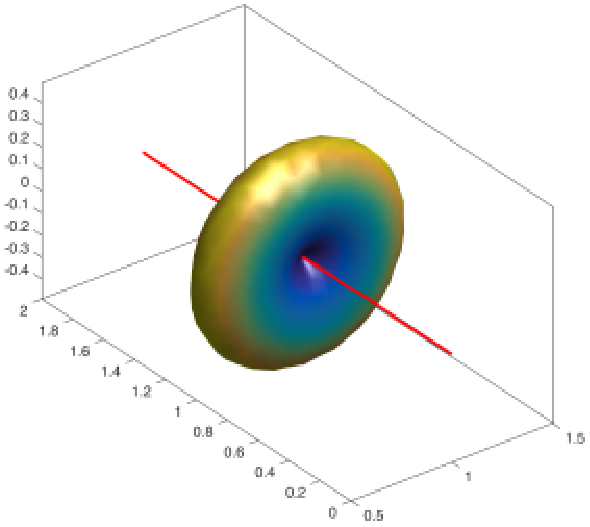
\includegraphics[width=0.3\columnwidth]{single_voxel_l.pdf}}
  \hspace*{0.7cm}
  \subfloat[ODF of (a)]{\label{subfig:line}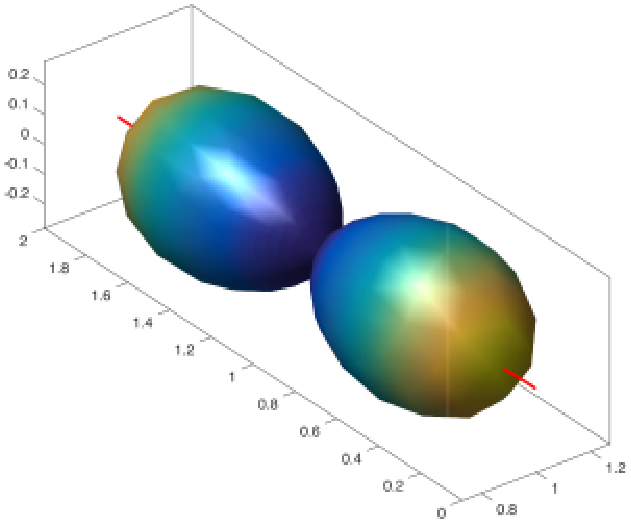
\includegraphics[width=0.3\columnwidth]{single_voxel_l_FRT.pdf}}\\
  \subfloat[HARDI
  sample]{\label{subfig:blob}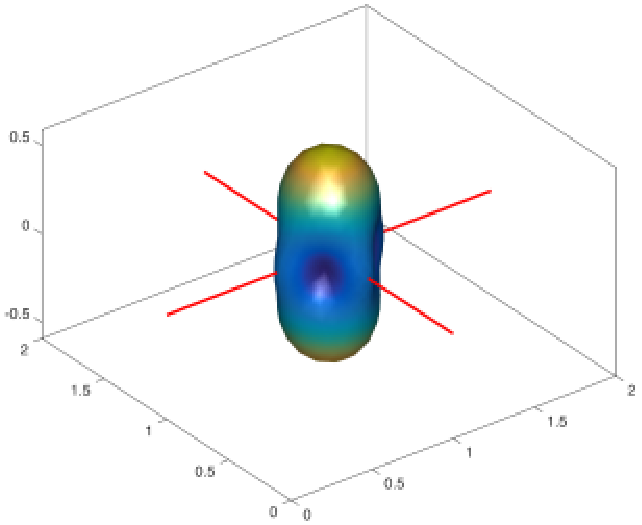
\includegraphics[width=0.45\columnwidth]{single_voxel_x.pdf}}
  \subfloat[ODF of
  (c)]{\label{subfig:cross}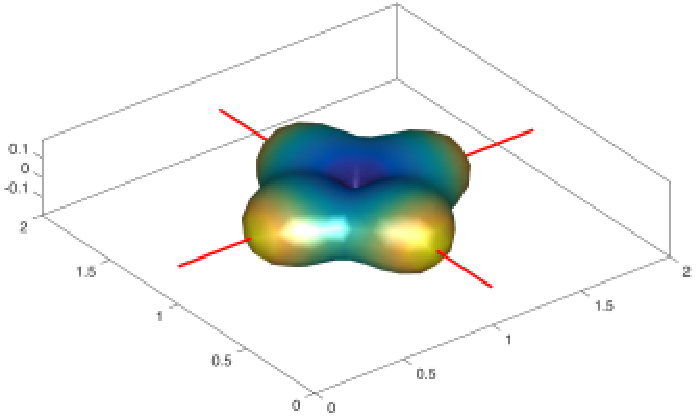
\includegraphics[width=0.45\columnwidth]{single_voxel_x_FRT.pdf}}
  \caption{Simulated DWI samples. The left column shows the raw DWI signal. The right
    column shows the reconstructed diffusion ODFs that follow anisotropic diffusion. The
    red lines indicate fiber orientations.}
  \label{fig:hardiandodf}
\end{figure}
These models can be combined to form simulated DWI tracts in various DWI shapes, such as
crossing fiber tracts \Cref{fig:crossingandnoise1}. A $20\times20$ grid is used throughout
this section to create blueprints of fiber tract constellations with the purpose of
performing LOR-DWI registrations. The images are coloured according to the generalized FA
(GFA) value where dark blue regions represent free isotropic diffusion. To simulate a more
realistic DWI scenario, random uniform noise has been added to the samples in
\Cref{fig:crossingandnoise1}.
\begin{figure}[!t]
  \centering
  \hspace*{-0cm}\subfloat[HARDI fiber tract crossing]{\label{subfig:crossnoise}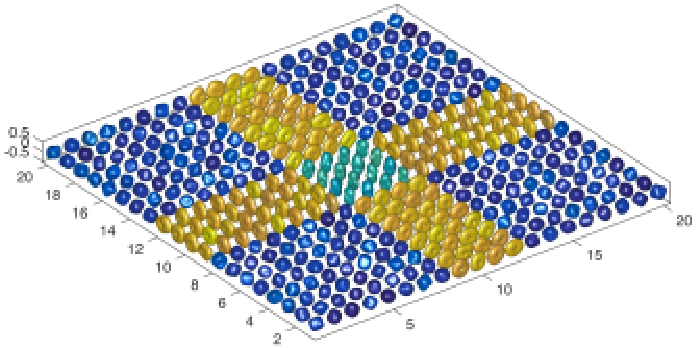
\includegraphics[width=1\columnwidth]{cross_default_n.pdf}}\\
  \hspace*{-0cm}\subfloat[ODFs of (a) showing the
  fibers]{\label{subfig:crossnoiseFRT}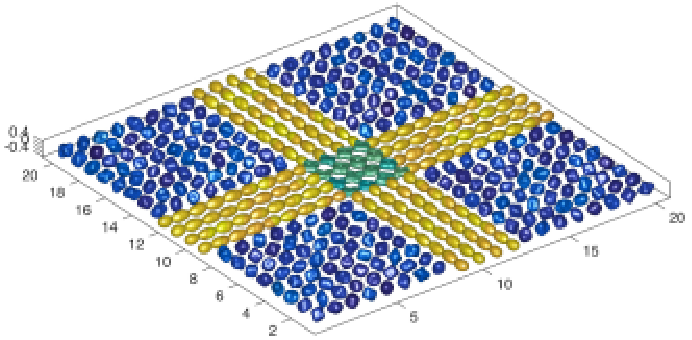
\includegraphics[width=1\columnwidth]{cross_default_n_FRT.pdf}}
  \caption{A simulated DWI fiber tract crossing with uniform random noise.}
  \label{fig:crossingandnoise1}
\end{figure}
The simulated voxels with unit density are rescaled for the free diffusion to have a low
density or mean diffusivity to resemble real $b_0$ normalized data.
\begin{figure}[!t]
  \centering \subfloat[HARDI fiber tract
  crossing]{\label{subfig:crossscaled}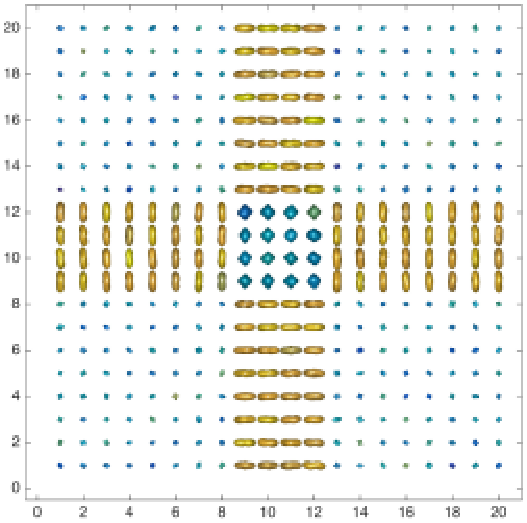
\includegraphics[width=0.475\columnwidth]{cross_default_ns.pdf}}
  \hspace*{.5cm}\subfloat[ODFs of (a) showing the
  fibers]{\label{subfig:crossscaledFRT}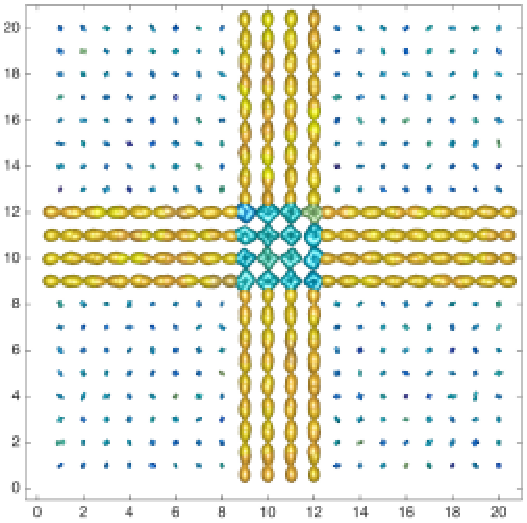
\includegraphics[width=0.475\columnwidth]{cross_default_ns_FRT.pdf}}
  \caption{Simulated DWI fiber tract crossing shown form above. The isotropic diffusion
    have now been normalized to have a lower mean diffusivity.}
  \label{fig:crossingandnoise3}
\end{figure}
\subsubsection{Parametric Setup}
For consistency the same setup is used for all experiments on the simulated data, unless
specifically stated otherwise.

\begin{description}
\item[Hierarchical mesh resolution.] In the B-spline deformation, the spacing between the
  control points is decreased in order to iteratively increase the degrees of freedom in
  the registration. We use
  $\Phi_{\text{local}} = \Phi_{\delta=4} + \Phi_{\delta=3.5} + \Phi_{\delta=3} +
  \Phi_{\delta=2}$.  10 iterations is used for all resolutions except the last, which
  terminates based on the optimal tolerance of $\epsilon = 1\mathrm{e}{-6}$, or 90
  iterations.
\item[Watson concentration, directional resolution.] The concentration parameter is set to
  $\kappa=15$, which is sufficiently smooth to represent the 100 uniform directions used.
\item[Spatial resolution.] A full spatial resolution is used with a B-spline smoothing at
  a near-Gaussian variance of $\sigma=0.6$ voxels.
\item[Histogram size.] Due to the relatively small data sample, a low number of bins is
  used for the histogram (i.e. intensity resolution) $20\times20$. This allows for some
  larger, stable but less refined deformations~\cite{darknersporring2012pami}.
\item[HARDI registration, ODF visualization.] We register the raw HARDI models but we
  visualize the ODFs of the warped data, based on the Funk-Radon transformed (FRT). We do
  this to illustrate that the warped raw data is correctly reoriented and \textit{do not}
  suffer visibly from affine shearing.
\item[Regularization.] We use regularization by a factor of $\lambda=1\mathrm{e}{-4}$. The
  regularization could have be omitted in the simulated experiments and substituted by
  multiple levels of resolution of the deformations (large to small), as the simulated
  data is very structured. As an aside, every example below could be highly improved by a
  experiment-specific choice of parameters, but for consistency the same settings were use
  for all experiments.
\end{description}

\subsection{Experiment 1: Single Fiber Tracts}
\label{subsec:singlefiber}
The first set of experiments are based on artificially generated distributions of HARDI
shells and corresponding ODFs, each representing different fiber constellations. The
experiment maps a straight fiber tract to a curved tract of the same width. It offers an
opportunity to discuss some of the differences between a good reconstruction and a correct
mapping.

\subsubsection{Straight and curved}

Three experiments illustrating the different scenarios where straight fibers are
registered to wavy fibers. These experiments illustrate the regularizing effects of using
the full diffusion profile for registration.  In the first experiment, the position of the
end of the fibers is constrained by adding intersecting fibers at the end and
beginning.\Cref{fig:straight2wavy_l} shows the simulated moving (straight) and target
(wavy) images.
\begin{figure}[!ht]
  \centering
  \vspace*{-0.4cm}
  \subfloat[Moving Image]{\label{subfig:straigt_l}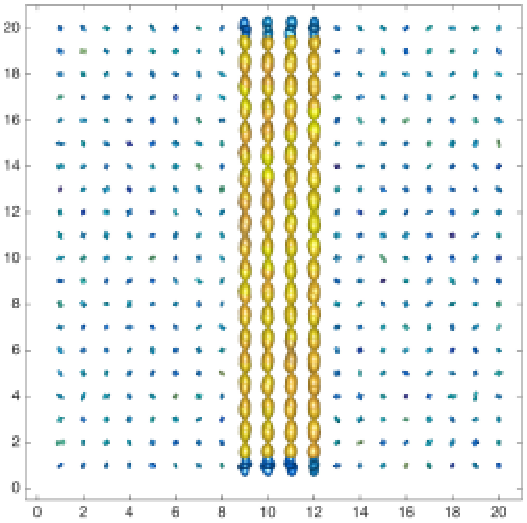
\includegraphics[width=0.475\columnwidth]{straight_l_FRT.pdf}}  
  \hspace*{.5cm}\subfloat[Target Image]{\label{subfig:wavy_l}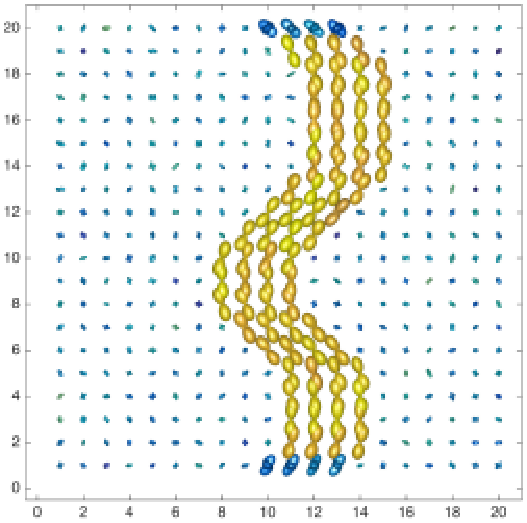
\includegraphics[width=0.475\columnwidth]{wavy_l_FRT.pdf}} 
  \caption{Experiment 1: Simulated fiber tract images with intersecting fibers at the boundaries.
  }
  \label{fig:straight2wavy_l}
\end{figure}
The results of the first experiment is shown in \Cref{fig:straight2wavy_l_results}, where
\ref{subfig:straigt2wavy_deform} is the reconstructed warp, and
\ref{subfig:straigt2wavy_arrows} shows the final spatial mapping from the moving image,
overlaid on the original target
image. 
As the figures illustrate the straight fibers are stretched in correspondence with the
curvature, and the reconstructed ODFs from the HARDI-based registration are rotated
correctly, although smoothed by the
interpolation.
\begin{figure}[!ht]
  \centering \vspace*{-0.4cm} \subfloat[Reconstructed warped
  image]{\label{subfig:straigt2wavy_deform}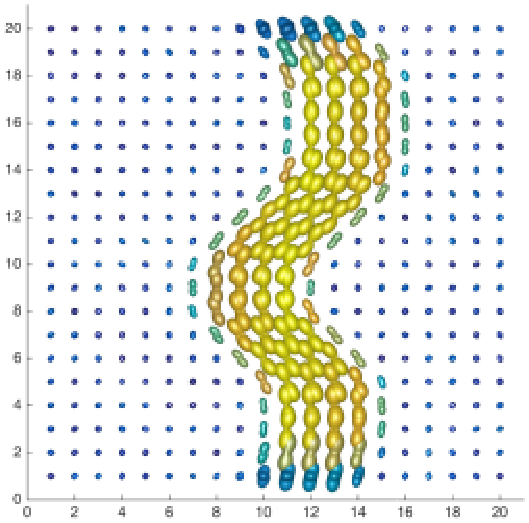
\includegraphics[width=0.475\columnwidth]{straight2wavy_FRT_deform.pdf}}
  \hspace*{.5cm}\subfloat[Spatial
  mapping]{\label{subfig:straigt2wavy_arrows}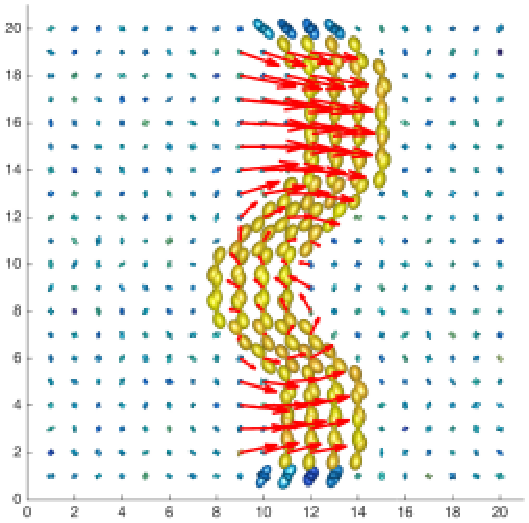
\includegraphics[width=0.475\columnwidth]{straight2wavy_FRT_arrows.pdf}}
  \caption{Experiment 1: Registration of single tract images of varying shape and (given
    the boundary) length.}
  \label{fig:straight2wavy_l_results}
\end{figure}
The second experiment is performed without features on the boundaries. The results are
shown in \Cref{fig:straight2wavy_l_boundary}, where we observe that the length is
preserved as the straight fiber tract is mapped to a sub-part of the curved
tract. Intuitively, a correct registration in such a case should preserve the length of
the straight fiber after deformation.
\begin{figure}[!ht]
  \centering \vspace*{-0.4cm} \subfloat[Reconstructed warped
  image]{\label{subfig:straigt2wavy_deform_boundary}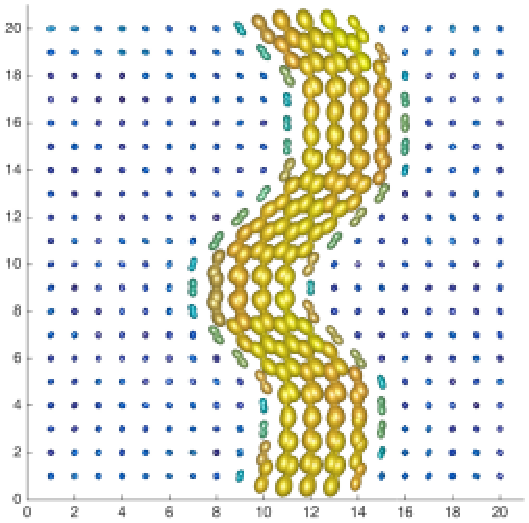
\includegraphics[width=0.475\columnwidth]{straight2wavy_noboundary_FRT_deform.pdf}}
  \hspace*{.5cm}\subfloat[Spatial
  mapping]{\label{subfig:straigt2wavy_arrows_boundary}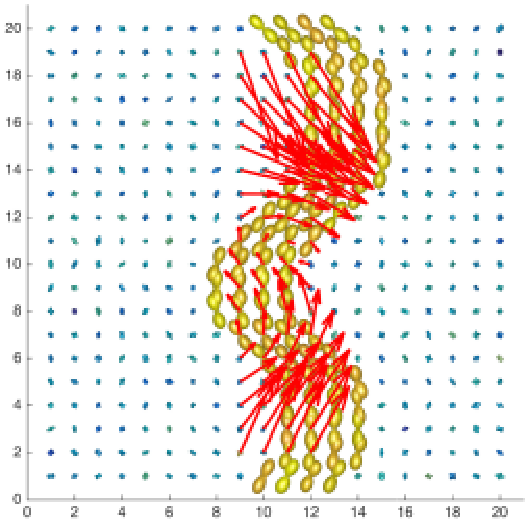
\includegraphics[width=0.475\columnwidth]{straight2wavy_noboundary_FRT_arrows.pdf}}
  \caption{Experiment 1: Registration of without boundary fibers. The spatial mapping
    indicates a nice preservation of length of the straight tract mapped to a subsection
    of the curved tract.}
  \label{fig:straight2wavy_l_boundary}
\end{figure}
The fact that this happens with no strong outside regularization, illustrate an inherent
regularization effect of the cost function.  In the third experiment, the proposed
similarity is compared with the equivalent scalar-based registration by performing a mean
diffusivity registration ($\kappa=0$) of the tracts with no signal on the boundaries. The
mean diffusivity carries no directional information. The result can be seen in
\Cref{fig:straight2wavy_l_boundary_k0}.
\begin{figure}[!ht]
  \centering \vspace*{-0.4cm} \subfloat[Reconstructed warped
  image]{\label{subfig:straigt2wavy_deform_boundary_k0}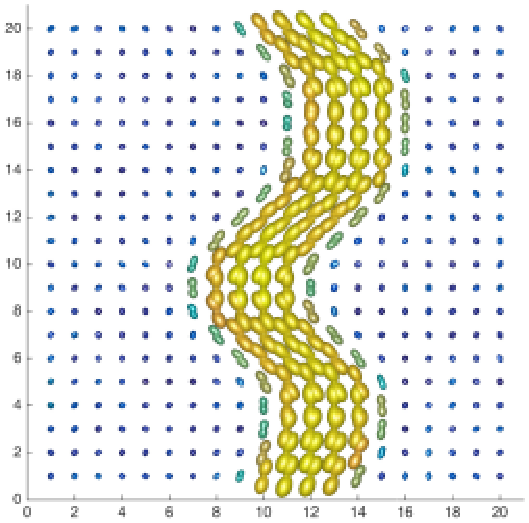
\includegraphics[width=0.475\columnwidth]{straight2wavy_noboundary_kappa0_FRT_deform.pdf}}
  \hspace*{.5cm}\subfloat[Spatial
  mapping]{\label{subfig:straigt2wavy_arrows_boundary_k0}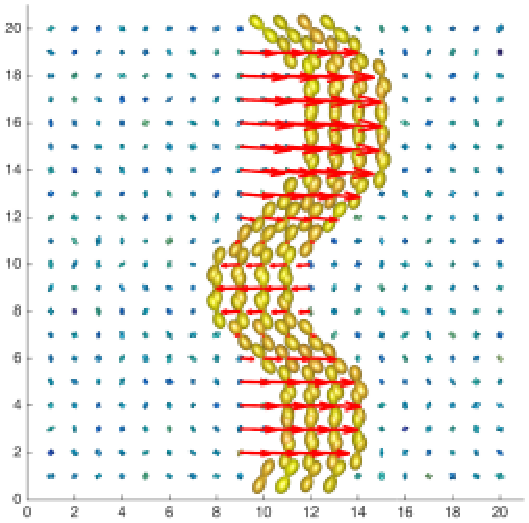
\includegraphics[width=0.475\columnwidth]{straight2wavy_noboundary_kappa0_FRT_arrows.pdf}}
  \caption{Experiment 1: Scalar-based registration without boundary fibers and no directional directional information in the cost function during optimization.}
  \label{fig:straight2wavy_l_boundary_k0}
\end{figure}
This pure scalar-based registration is driven by the edges of the simulated tracts
only. The reconstruction appears to be correct, but the final spatial mapping indicates a
lack of regularization as the fibers are stretched
unevenly.


\subsection{Experiment 2: Crossing Fiber Tracts}
\label{subsec:crossingfiber}

The second set of experiments are designed to investigate the registration of crossing fiber tracts.

\subsubsection{Straight and shifted}

The first experiment examines the framework's ability to register two crossing tracts with
a horizontal and vertical shift
\Cref{subfig:straight_x_2shift,subfig:straight_x_shifted}. Circular fibers have been added
as fixed points in the image to illustrate the local shift of the crossing tracts. The
result of the registration is shown in
\Cref{subfig:straigt2shift_deform,subfig:straigt2shift_arrows}. The final spatial mapping,
shown with arrows, is accurate including the reconstruction. Note that the reconstruction
is subject to the effect of the smoothing in the interpolation.

\subsubsection{Two degrees of shearing}

The second experiment involving crossing fibers show three fiber tracts crossing under a
varying amount of shear with a fixed horizontal tract (
\Cref{subfig:sheared30,subfig:sheared40}). The purpose is to investigate a relatively
large deformation combined with a change to the complex crossing at the center. The
results are shown in \Cref{subfig:sheared_deform,subfig:sheared_arrows}. As the figure
illustrates the structure of the complex center-crossing closely matches the orientations
of 45 degree crossing fibers. We remind the reader that the registration was not performed
on the ODFs but directly on the simulated HARDI models and subsequently reconstructed.

\subsection{Experiment 3: Fanning Fiber Tracts}
\label{subsec:kissingfiber}

The third set of experiments examines the most complex configurations namely the
registration of kissing and fanning fibers. Note that although the artificial cases
constructed for these experiments have a 1-1 correspondence.

\subsubsection{Fanning and kissing fiber tracts in a crossing}

The first experiment consist of two DWI images, that simulates both fanning (dispersing)
and kissing (interleaving) fiber tracts. The moving image in
\Cref{subfig:fanning,subfig:kissing} contains a crossing with a few fibers fanning in and
out along the vertical center line. The target image contains two curved tracts fanning in
and out, and merging at the central crossing. The results of the registration experiment
are shown in \Cref{subfig:fanning_deform,subfig:kissing_arrows}, where both the
reconstructed warp and spatial mapping show a registration that follows the lines of the
original target image. The resulting registration is able to move, shrink and turn the
center-crossing to fit to fit the target image.

\subsubsection{Kissing fiber tracts}

The second experiment involves two straight fiber tracts that are registered to two
curving and interleaving tracts (\Cref{subfig:straightlines,subfig:kissinglines}).  The
result, shown in \Cref{subfig:straight2kiss_deform,subfig:straight2kiss_arrows}, displays
a large and difficult deformation that by all accounts appears to be a successful
registration.

%% %% %% %% %% %% %% %% %% %% %% %%
%% 4 rows of experiment figures  %%
%% %% %% %% %% %% %% %% %% %% %% %%
\begin{figure*}[!t]
  \centering \subfloat[Moving
  Image]{\label{subfig:straight_x_2shift}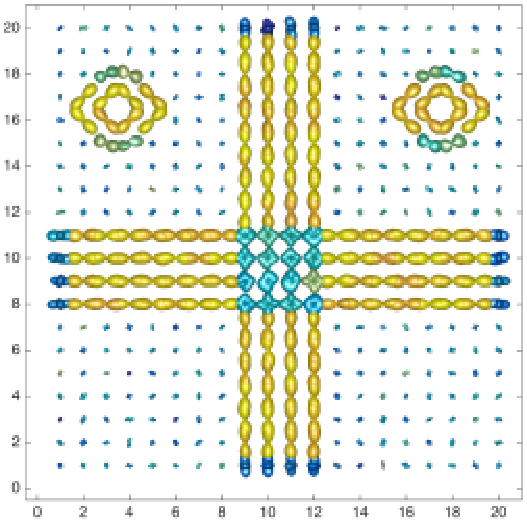
\includegraphics[width=0.5\columnwidth]{straight_x_FRT.pdf}}
  \hspace*{.1cm}\subfloat[Target
  Image]{\label{subfig:straight_x_shifted}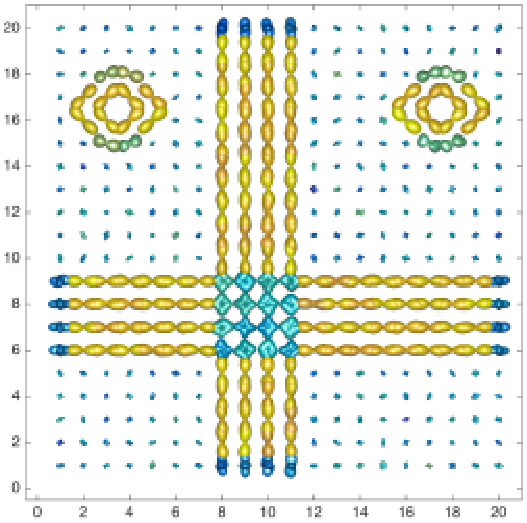
\includegraphics[width=0.5\columnwidth]{shifted_x_FRT.pdf}}
  \hspace*{.1cm}\subfloat[Reconstructed warped
  image]{\label{subfig:straigt2shift_deform}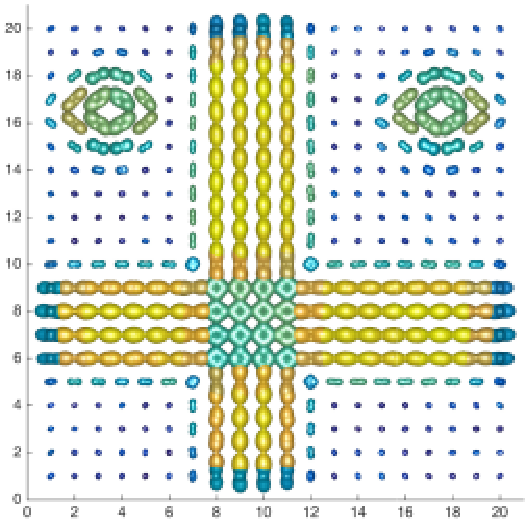
\includegraphics[width=0.5\columnwidth]{straigt2shift_FRT_deform.pdf}}
  \hspace*{.1cm}\subfloat[Spatial
  mapping]{\label{subfig:straigt2shift_arrows}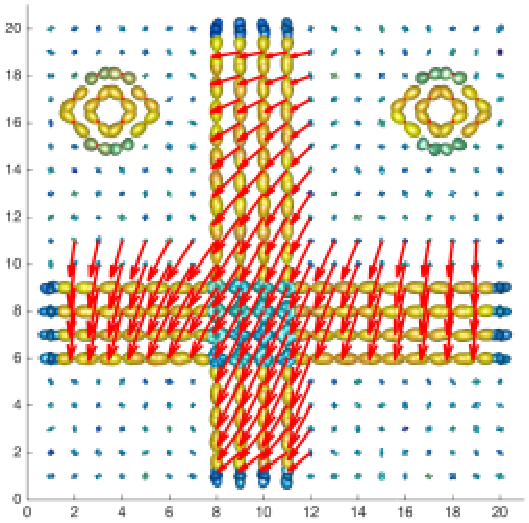
\includegraphics[width=0.5\columnwidth]{straigt2shift_FRT_arrows.pdf}}
  \caption{Experiment 2: Simulated crossing tracts (a) with a vertical shift (b). The
    registered result of the crossing under a both vertical and horizontal shift is
    reconstructed in (c), and shown with the final spatial mapping from the original
    position of the moving image in (d).}
  \label{fig:straight2shift_x_results}
  \vspace*{-0.5cm}
\end{figure*}
\begin{figure*}[!t]
  \centering \subfloat[Moving
  Image]{\label{subfig:sheared30}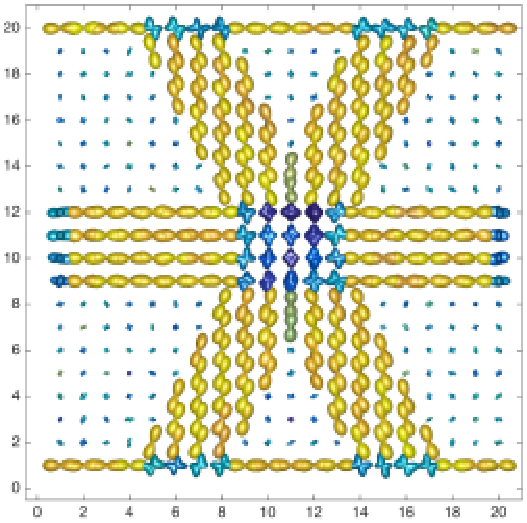
\includegraphics[width=0.5\columnwidth]{sheared30_x_FRT.pdf}}
  \hspace*{.1cm}\subfloat[Target
  Image]{\label{subfig:sheared40}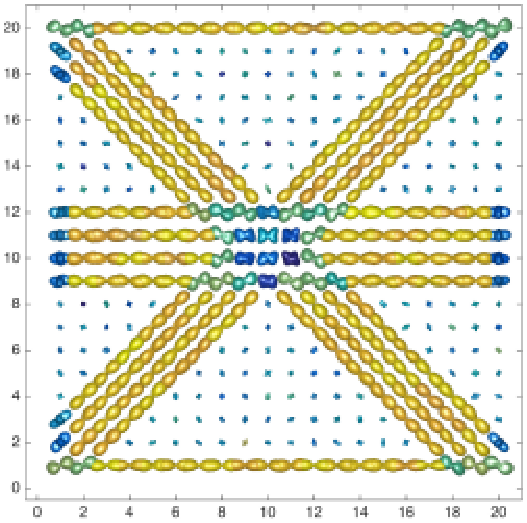
\includegraphics[width=0.5\columnwidth]{sheared45_x_FRT.pdf}}
  \hspace*{.1cm}\subfloat[Reconstructed warped
  image]{\label{subfig:sheared_deform}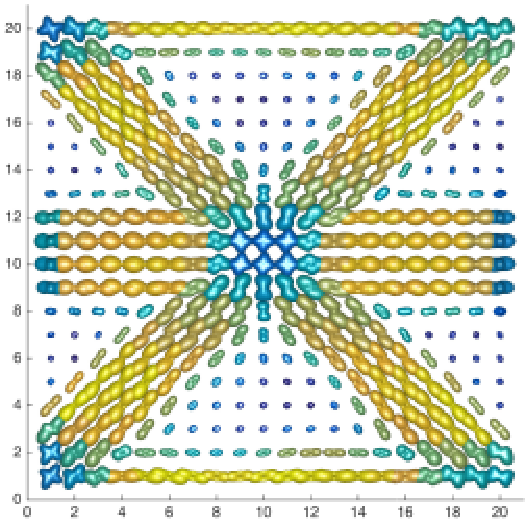
\includegraphics[width=0.5\columnwidth]{sheared2sheared_FRT_deform.pdf}}
  \hspace*{.1cm}\subfloat[Spatial
  mapping]{\label{subfig:sheared_arrows}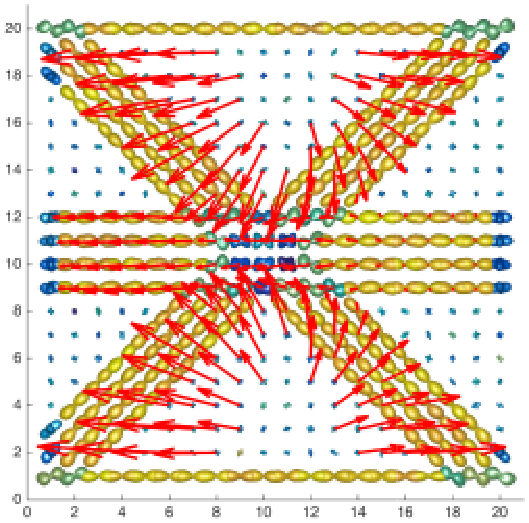
\includegraphics[width=0.5\columnwidth]{sheared2sheared_FRT_arrows.pdf}}
  \caption{Experiment 2: Simulated crossing tracts with $\sim$30 degree (a) to 45 degree
    shearing (b). The reconstruction of the registered result is shown in (c), and the
    corresponding spatial mapping in (d).}
  \label{fig:sheared2sheared_x_results}
  \vspace*{-0.5cm}
\end{figure*}
\begin{figure*}[!t]
  \centering \subfloat[Moving
  Image]{\label{subfig:fanning}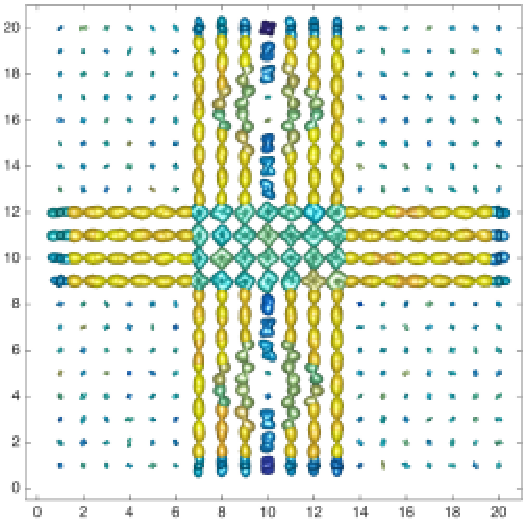
\includegraphics[width=0.5\columnwidth]{complex_thick_FRT.pdf}}
  \hspace*{.1cm}\subfloat[Target
  Image]{\label{subfig:kissing}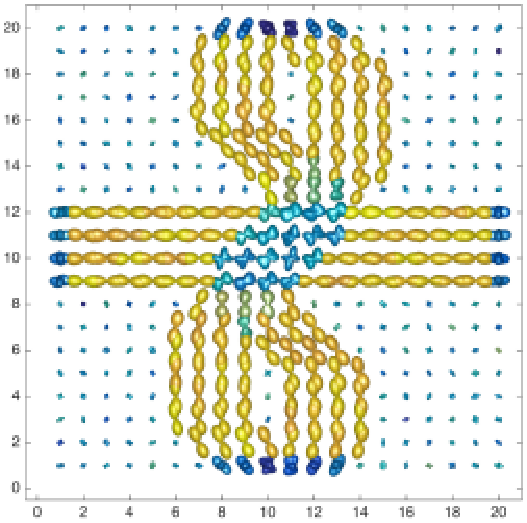
\includegraphics[width=0.5\columnwidth]{complex_wavy_FRT.pdf}}
  \hspace*{.1cm}\subfloat[Reconstructed warped
  image]{\label{subfig:fanning_deform}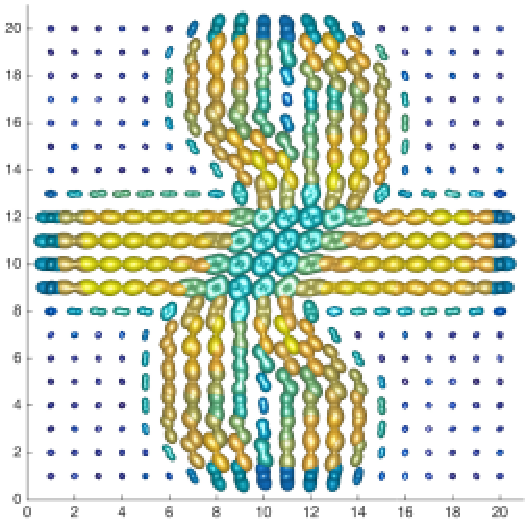
\includegraphics[width=0.5\columnwidth]{complex_FRT_deform.pdf}}
  \hspace*{.1cm}\subfloat[Spatial
  mapping]{\label{subfig:kissing_arrows}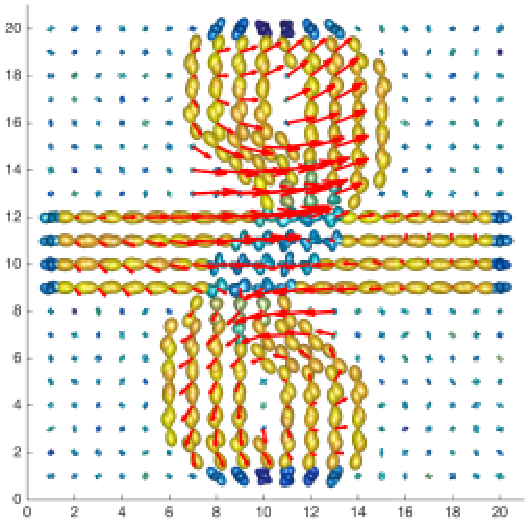
\includegraphics[width=0.5\columnwidth]{complex_FRT_arrows.pdf}}
  \caption{Experiment 3: (a) Simulated fanned opening in the moving image, and (b) an
    interleaving curved target image. The reconstruction is shown in (c), and the spatial
    mapping in (d).}
  \label{fig:fanning2kissing_x_results}
  \vspace*{-0.5cm} 
\end{figure*}
\begin{figure*}[!t]
  \centering \subfloat[Moving
  Image]{\label{subfig:straightlines}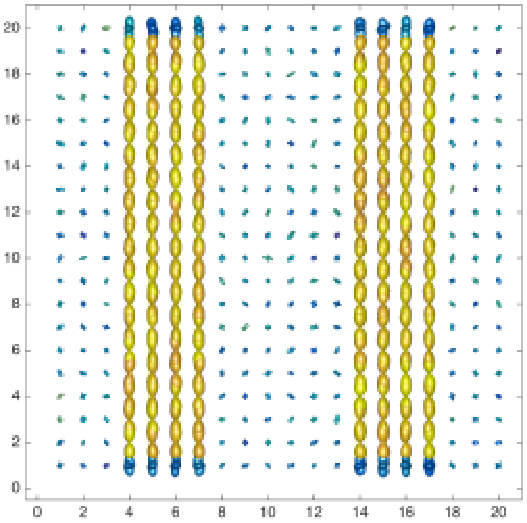
\includegraphics[width=0.5\columnwidth]{straight_ll_FRT.pdf}}
  \hspace*{.1cm}\subfloat[Target
  Image]{\label{subfig:kissinglines}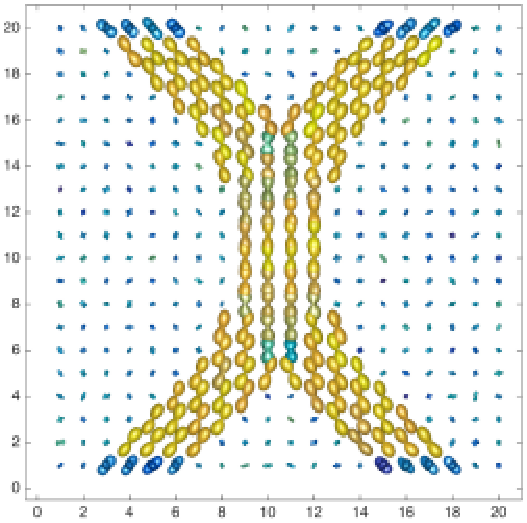
\includegraphics[width=0.5\columnwidth]{kissing_ll_FRT.pdf}}
  \hspace*{.1cm}\subfloat[Reconstructed warped
  image]{\label{subfig:straight2kiss_deform}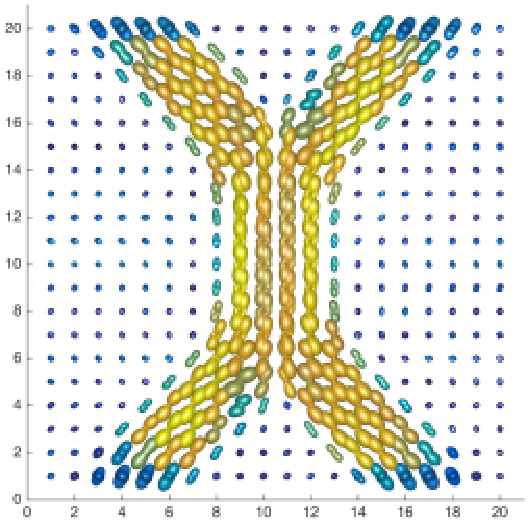
\includegraphics[width=0.5\columnwidth]{kissing_ll_FRT_deform.pdf}}
  \hspace*{.1cm}\subfloat[Spatial
  mapping]{\label{subfig:straight2kiss_arrows}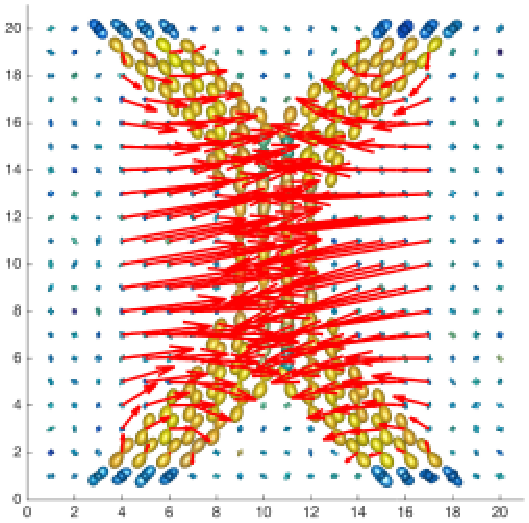
\includegraphics[width=0.5
    \columnwidth]{kissing_ll_FRT_arrows.pdf}}
  \caption{Experiment 3: Simulated straight (a) and kissing (b) fiber tracts. The
    reconstruction is shown in (c), and the spatial mapping in (d).}
  \label{fig:straight2kiss_results}
\end{figure*}


\subsection{Synthetic Deformations of Real Data}
\label{sec:syndeform}

In this set of experiments, the registration framework is evaluated on real data obtained
from the HCP \cite{van2013wu}. By introducing a random synthetic warp on a subset of the
brain data, a ground truth is obtained where the objective is to register the warped image
back to the original image. These experiments illustrate the effect of the parameters of
the model in a realistic scenario in a guaranteed diffeomorphic
scenario.

\subsubsection{DWI example data}

\begin{figure}[H]
  \centering
  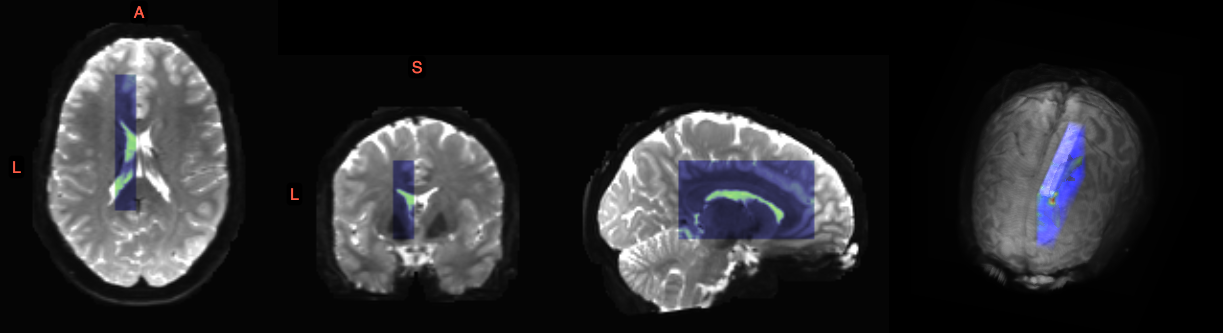
\includegraphics[width=1\columnwidth]{B0_roi_overlay.png}
  \caption{Selected region of interest for synthetic warp experiments (blue) overlaid on
    the $b_0$ image of HCP subject \texttt{103818}.}
  \label{fig:cc_roi_b0}
\end{figure}
The DWI data used in this experiment is shown in \Cref{fig:cc_roi_b0}, where the region of
interest (ROI) is the blue overlay on the subjects $b_0$ image. An ROI of the brain is
used to improve the visualization of the results. The ROI was chosen at the edge of the
corpus callosum (CC) in the left hemisphere due to the characteristic C-shape of the CC
and the intersection with other well-known structures e.g. the cingulum. Furthermore, the
ROI is in an area with crossing fiber tracts and is near the cortex. A $b=1000$ DWI volume
is used with the ROI being $11\times71\times41$ at 1.25mm isotropic voxels with 90
directions. Only the central sagittal slice along with corresponding ODFs is visualised
(\Cref{subfig:cc_slice}), while the deformation is applied to the whole ROI. The
deformation field for the central slice is shown in \Cref{subfig:cc_deform}.

\begin{figure}[ht]
  \centering
  \subfloat[Sagittal slice at ROI center.]{\label{subfig:cc_slice}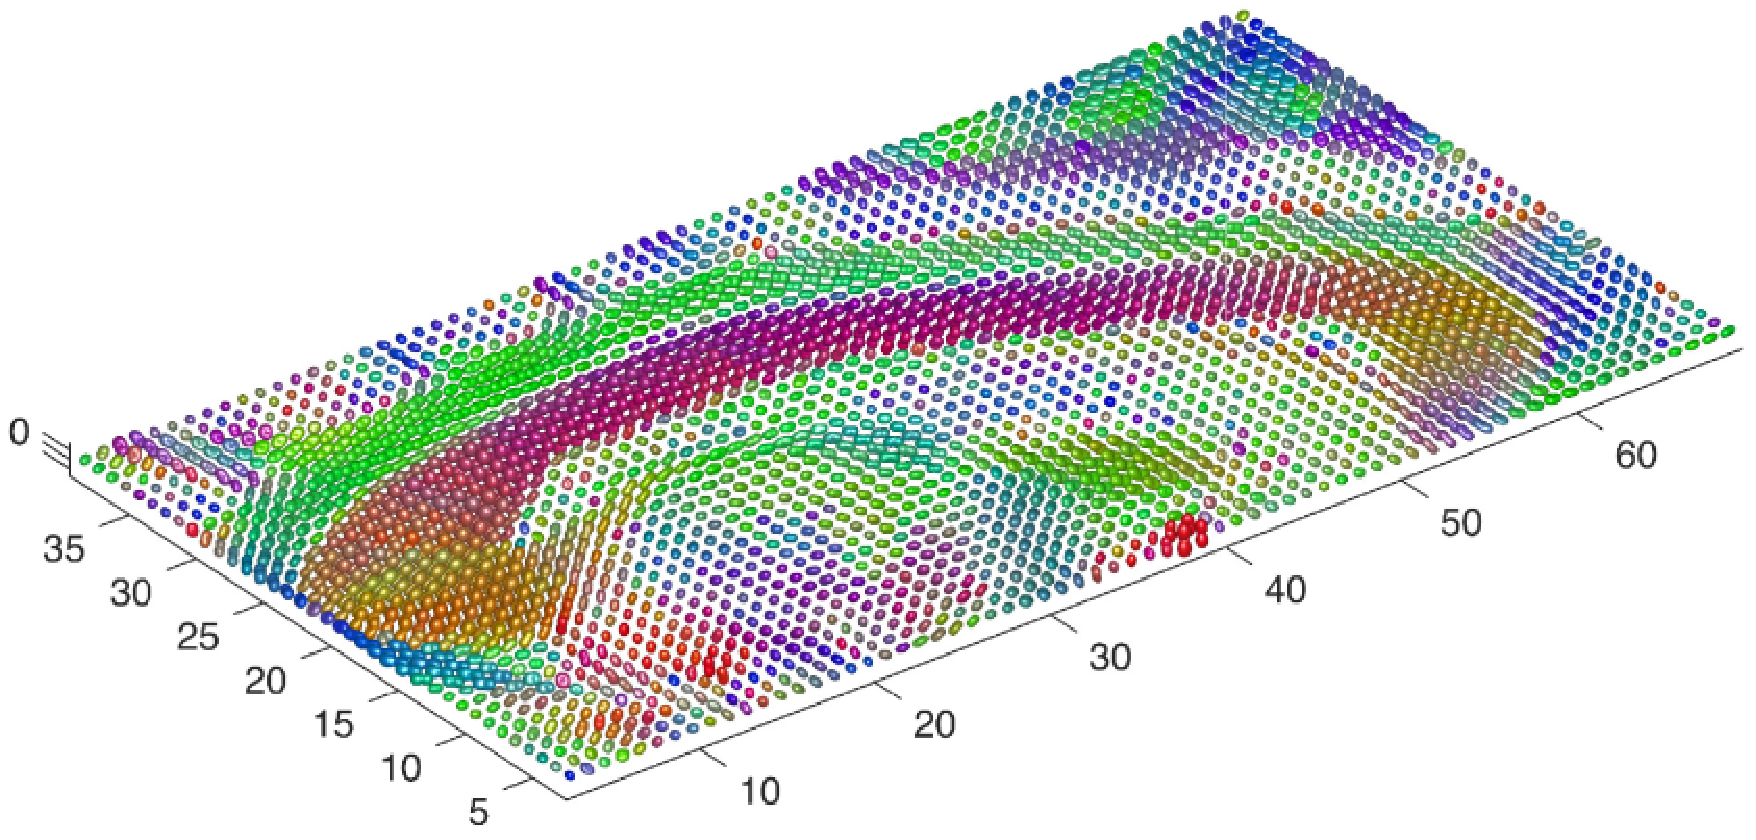
\includegraphics[width=1\columnwidth]{CC_slice_orig.pdf}}\\
  \subfloat[Deformation
  field.]{\label{subfig:cc_deform}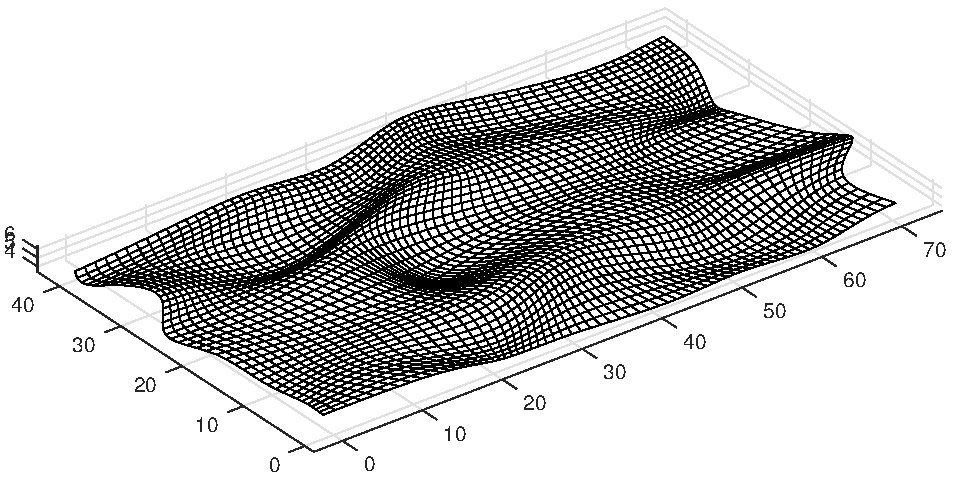
\includegraphics[width=1\columnwidth]{deformattionfield.pdf}}
  \caption{Original central ROI slice with ODFs (a), and the deformation to be applied
    (b).}
  \label{fig:cc_slice2}
\end{figure}

\subsubsection{The effects of the parameters}
The experimental setup provides a ground truth, which is simply the identity
transformation. As the similarity measure, NMI, does not reflect a unique point-wise
correspondence, we introduce three measures for evaluating the resulting registration: (1)
mean squared error (MSE) between coordinates, (2) curl of the final deformation field, and
(3) divergence of the final deformation field \cite{helmholz1858}.

\textit{Curl}
quantifies the amount of orientational change in the deformation field, also referred to
as rotation or vorticity. We use the $L_2$-norm of the curl vector, i.e. the velocity of
rotation. A higher magnitude of the curl is expected for the results of a scalar-based
registration compared to a registration over the full diffusion profile.


\textit{Divergence} quantifies the density of the outward flux of a vector field which can
be either positive or negative, indicating an expansion or a contraction at a given
point. %
In combination, these three measures provide information about the magnitude of the
voxel-wise distance and the state of the final deformation field. Curl and divergence has
previously been used as regularization in a nonrigid registration framework
\cite{riyahi2014regularization}.

In the following, the experiments are performed while varying the intensity scale, the
orientation scale, and the spatial scale, as it is the intensity and orientational scale
that sets this registration framework apart form other frameworks. The following is
investigated:
\begin{description}
\item[1. Isointensity curves.] The density-based formulation allows us to smooth the image
  inverse proportionally to the image gradients, such as the borders near the CSF, which
  can be strongly affected by partial volume effects. We iteratively decrease the control
  point-spacing in the FFD model to get an increasingly localized registration, and
  increase the intensity range accordingly. This is realized with an initial histogram
  with relatively few bins and a fixed degree of smoothing and then successively increase
  the number of bins as the deformation resolution is increased of iterations.
\item[2. Explicit reorientation.] The directional information is, according to our
  experiments, expected to provide a more stable and regularized transformation. To
  investigate this hypothesis, different levels of directional smoothing are examined from
  $\kappa=30$ a highly peaked ODF to a scalar-based mean diffusivity registration
  i.e. setting the concentration parameter $\kappa$ to $0$. The experiments on simulated
  data indicated that the directional information results in direct regularized solutions
  through the similarity, and these experiments seek to uncover if these observations hold
  for real data.
\end{description}
Performing multi-resolution registration (a continuation method) is a key element in most
high resolution registration frameworks, e.g. in the FFD model
\cite{rueckert1999nonrigid}, \texttt{ANTs} \cite{avants2009advanced}, \texttt{Elastix}
\cite{klein2010elastix}, \texttt{FSL} \cite{jenkinson2012fsl}, etc. It provides stability
while allowing for large and small deformations while reducing the computational
complexity. While experiments regarding the spatial part will be performed, its impact on
registration quality is fairly well-described in contrast to iso-intensity curves and
explicit reorientation.

\subsubsection{Parametric Setup}

\begin{description}
\item[Hierarchical mesh resolution.] Similar to the simulated experiments, the spacing
  between the control points is successively decreased. To this end we use the composition
  $\Phi_{\text{local}} = \Phi_{\delta=10} \circ \Phi_{\delta=5} \circ \Phi_{\delta=3.5}
  \circ \Phi_{\delta=3}$, where the control point spacing $\delta$ is scaled down
  according to the dimensions of the image. The low initial resolution of the deformation
  permits the generation of a large random and valid synthetic warp at around half of the
  control point spacing ($\sim$ $0.4\delta$) \cite{rueckert2006diffeomorphic}. For the
  optimization we use a quasi-Newton L-BFGS optimizer which runs for 50 iterations for all
  resolutions, unless the optimality condition of $\epsilon = 1\mathrm{e}{-6}$ is
  fulfilled. Note that we refer to the result after each optimizer termination as
  \textit{a step}, thus 4 steps in total.
\item[Accumulated curl and divergence.] While the MSE is easy to calculate at each step,
  the curl and divergence depend on the first-order derivatives of the spatial
  deformation, which are accumulated over each step. Thus the final curl and divergence is
  defined by the product of Jacobians for each step
  $Curl(\Phi_{\delta=3}) = \bm J(\Phi_{\delta=10})\bm J(\Phi_{\delta=5})\bm
  J(\Phi_{\delta=3.5})\bm J(\Phi_{\delta=3})$ for all voxels.
\item[Change in resolution.] Changing spatial resolution is achieved by convolution.
\item[Other fixed parameters.] The regularization is fixed to $\lambda=1\mathrm{e}{-4}$,
  and we interpolate and optimize over 30 interpolated orientations of the 90 in the HCP
  data.
\end{description}
All the following experiments will show results of the four accumulating steps. All error
measures are reported for the entire ROI and not just the slice visualized.

\subsubsection{The Quantitative Effect of Isoparametric Curves}
\label{subsec:isocurvesparam}

This experiment illustrates the effect of changing the size of the smoothed joint
histogram. Three experiments are performed with (i) a fixed histogram of $50\times50$
bins, (ii) a histogram with $500\times500$ bins, and (iii) gradually increasing the
histogram size in 50, 100, 200 and 500 bins. \Cref{fig:binstest} shows the results in
terms of MSE, curl and divergence as mean value over all points along.
\begin{figure*}[!htb]
  \centering
  \hspace*{0cm}\subfloat[MSE]{\label{subfig:binsmse}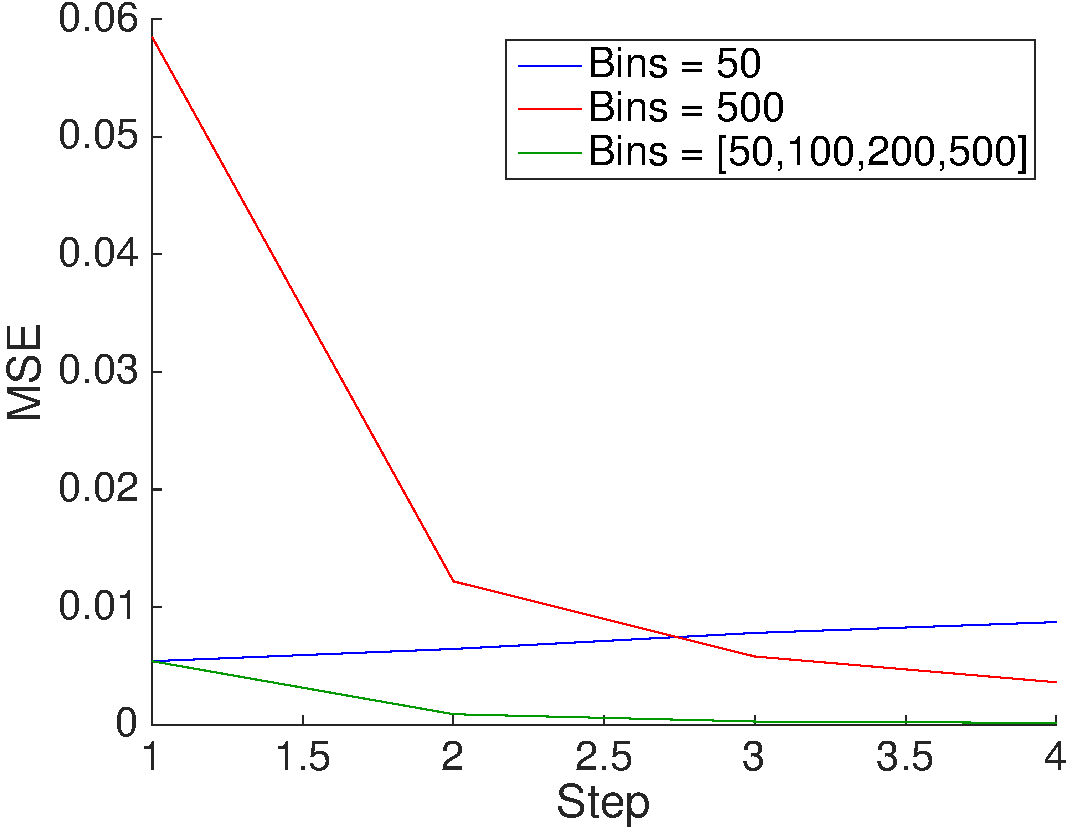
\includegraphics[width=0.60\columnwidth]{bins_mse.pdf}}
  \hspace*{0cm}\subfloat[Curl]{\label{subfig:binscurl}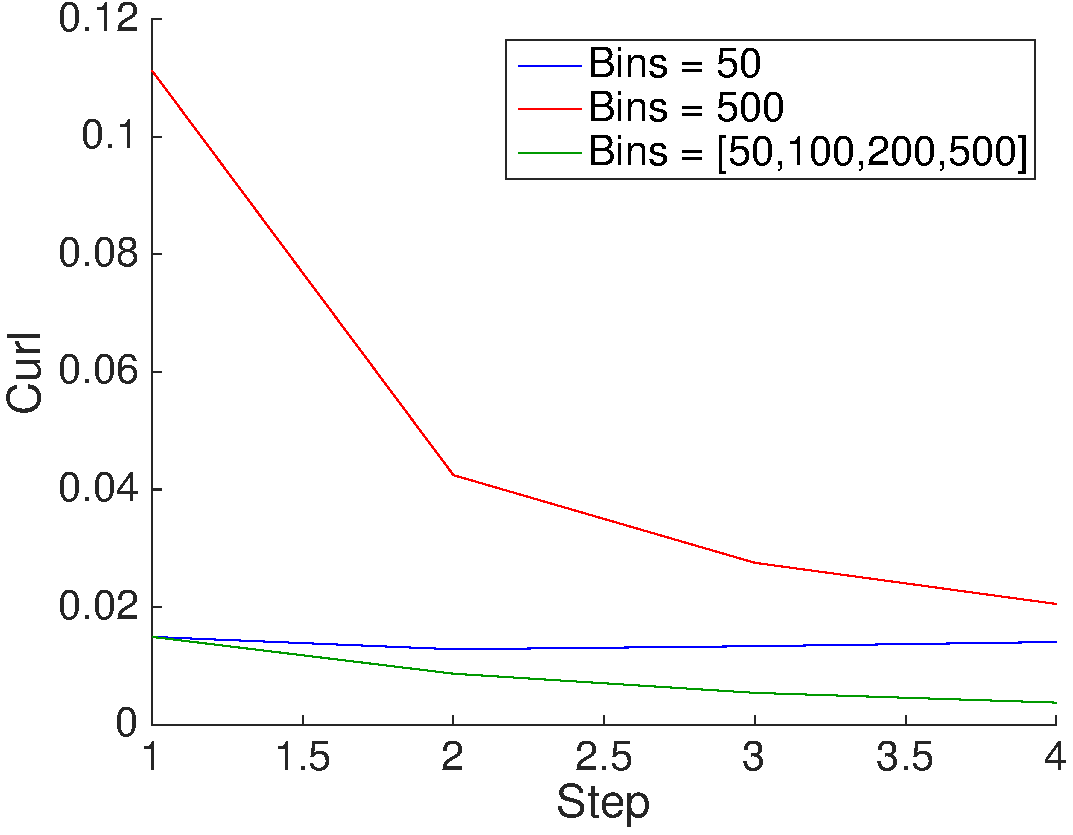
\includegraphics[width=0.60\columnwidth]{bins_curl.pdf}}
  \subfloat[(Absolute)
  Divergence]{\label{subfig:binsdiv}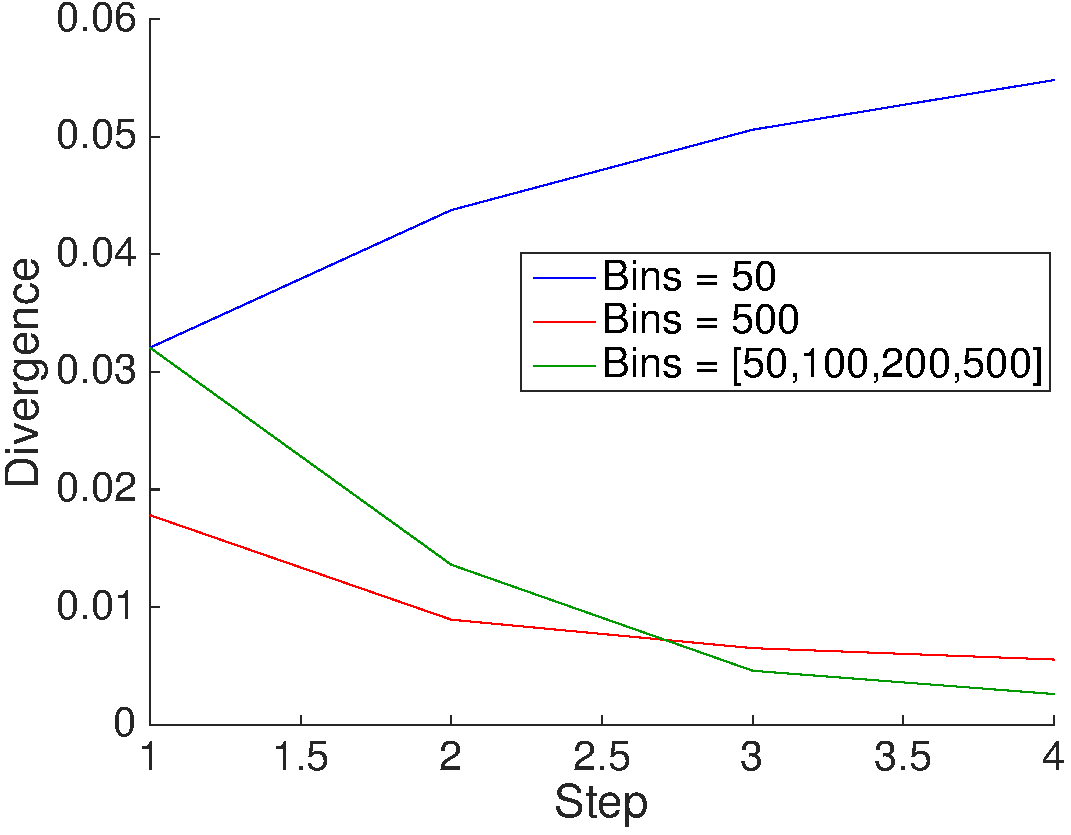
\includegraphics[width=0.60\columnwidth]{bins_div.pdf}}
  \caption{Results from testing the effect of the number of bins through the four step
    registration. The lines are the mean over all points. The best results are (a): green
    at $1.42\mathrm{e}{-4}$, (b): green at $3.74\mathrm{e}{-3}$, and (c): green at
    $2.60\mathrm{e}{-3}$.}
  \label{fig:binstest}
\end{figure*}
It is evident how a small histogram with wide isocurves results in an initially faster
convergence \Cref{fig:binstest} (blue line). However, wide iso-curves result in flat
regions with small gradients and little structure which may cause the result to become
sub-optimal or degenerate with increasing degrees of freedom in the transformation. In
contrast, starting with a high-resolution of the histogram with thin iso-curves has the
opposite effect in the initial steps (red line). However, by iteratively refining the
joint histogram, we allow for a wide to thin movement in the image, which provides
superior result (green line).

\subsubsection{The Quantitative Effect of the Orientation Scale}
\label{subsec:orientationparam}

In this experiment, we investigate if directional information increases the stability and
improves the registration. We employ the size progression of the histogram from the
previous experiment (i.e. [50,100,200,500]), and vary the concentration parameter $\kappa$
from mean diffusivity at $\kappa=0$ to sharp angular features at $\kappa=30$. The results
are shown in \Cref{fig:kappatest}.
\begin{figure*}[!htb]
  \centering
  \hspace*{0cm}\subfloat[MSE]{\label{subfig:kappamse}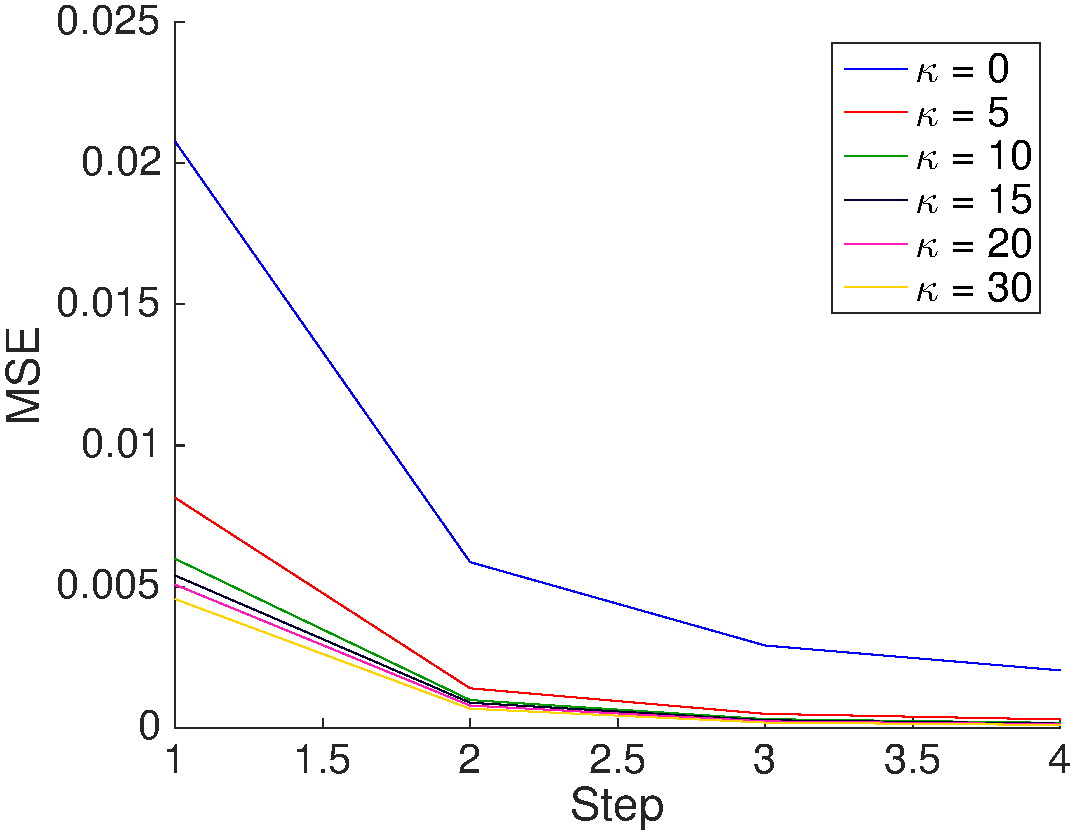
\includegraphics[width=0.60\columnwidth]{kappa_mse.pdf}}
  \hspace*{0cm}\subfloat[Curl]{\label{subfig:kappacurl}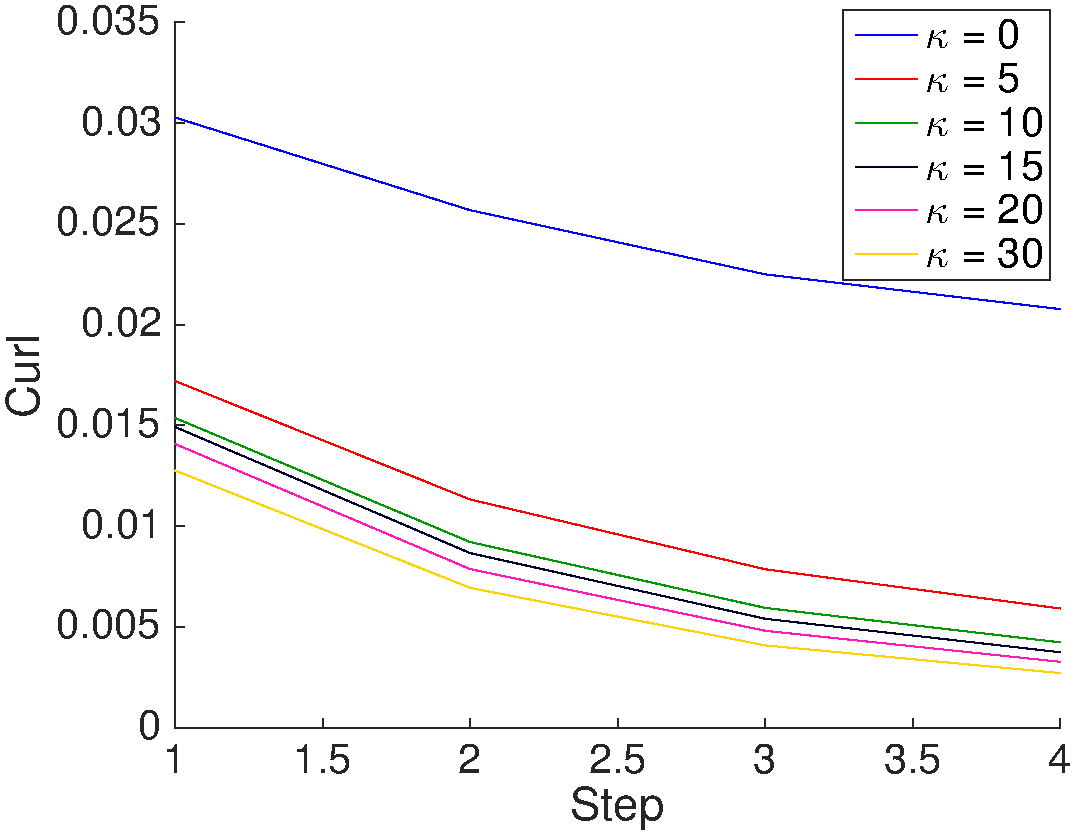
\includegraphics[width=0.60\columnwidth]{kappa_curl.pdf}}  
  \subfloat[(Absolute) Divergence]{\label{subfig:kappadiv}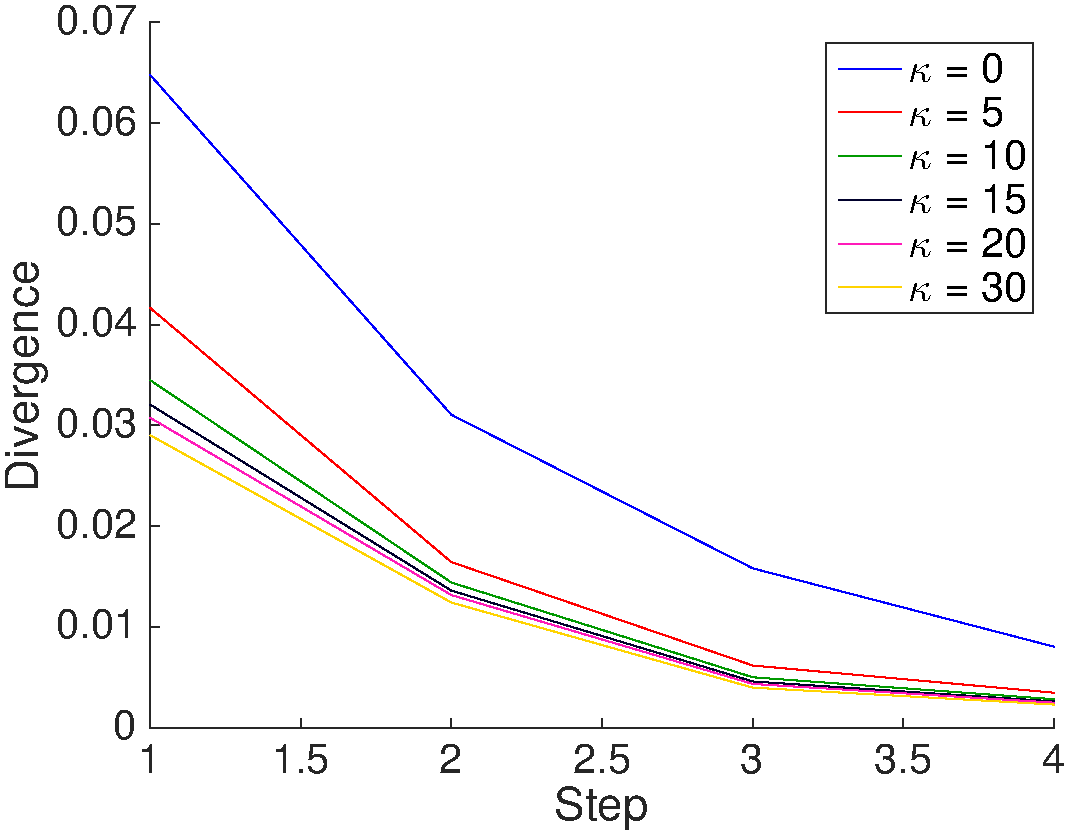
\includegraphics[width=0.60\columnwidth]{kappa_div.pdf}}
%  \vspace*{0.5cm} 
  \caption{Results from testing the effect of smoothness of the directional interpolation
    through the four step registration. The lines are the mean over all points. The best
    results are the yellow line at $\kappa=30$ with (a): $9.17\mathrm{e}{-5}$, (b):
    $2.71\mathrm{e}{-3}$, and (c): $2.29\mathrm{e}{-3}$. However, the overall difference
    between $\kappa=10$ and $\kappa=30$ is not more than around $1\mathrm{e}{-5}$.}
  \label{fig:kappatest}
\end{figure*}
The figure shows how the directional information results in better registration, with
significantly less curl than the scalar registration at $\kappa=0$ and we observe that the
best value $\kappa=30$ is stable in high directional resolution data such as the HCP. We
suggest setting $\kappa=15$ as this is should suffice for both high and low resolution
data, such as DTI.

\subsubsection{The Quantitative Effect of the Spatial Resolution}
\label{subsec:spatialparam}

In the last experiment, we use $\kappa=15$, set the bins to $[50,100,200,500]$, and
investigate the effects of changing the spatial scale.
\begin{figure*}[!htb]
  \centering
  \hspace*{0cm}\subfloat[MSE]{\label{subfig:spatialmse}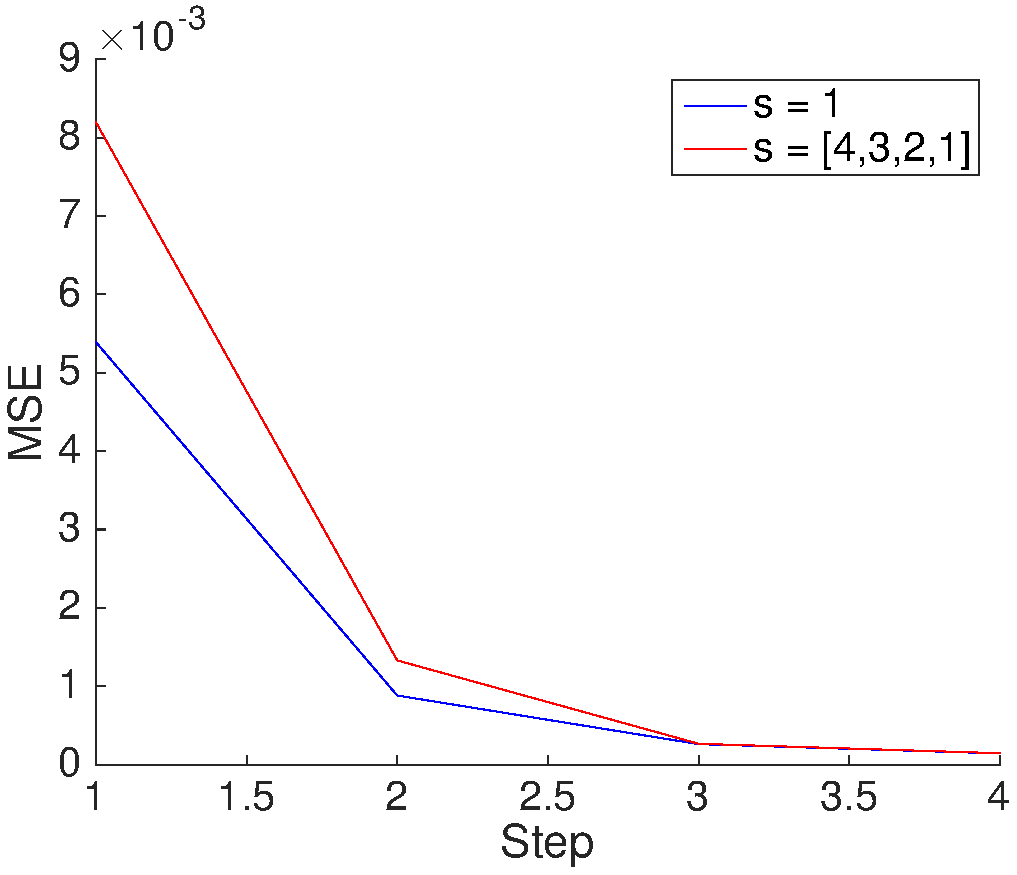
\includegraphics[width=0.55\columnwidth]{spatial_mse.pdf}}
  \hspace*{0cm}\subfloat[Curl]{\label{subfig:spatialcurl}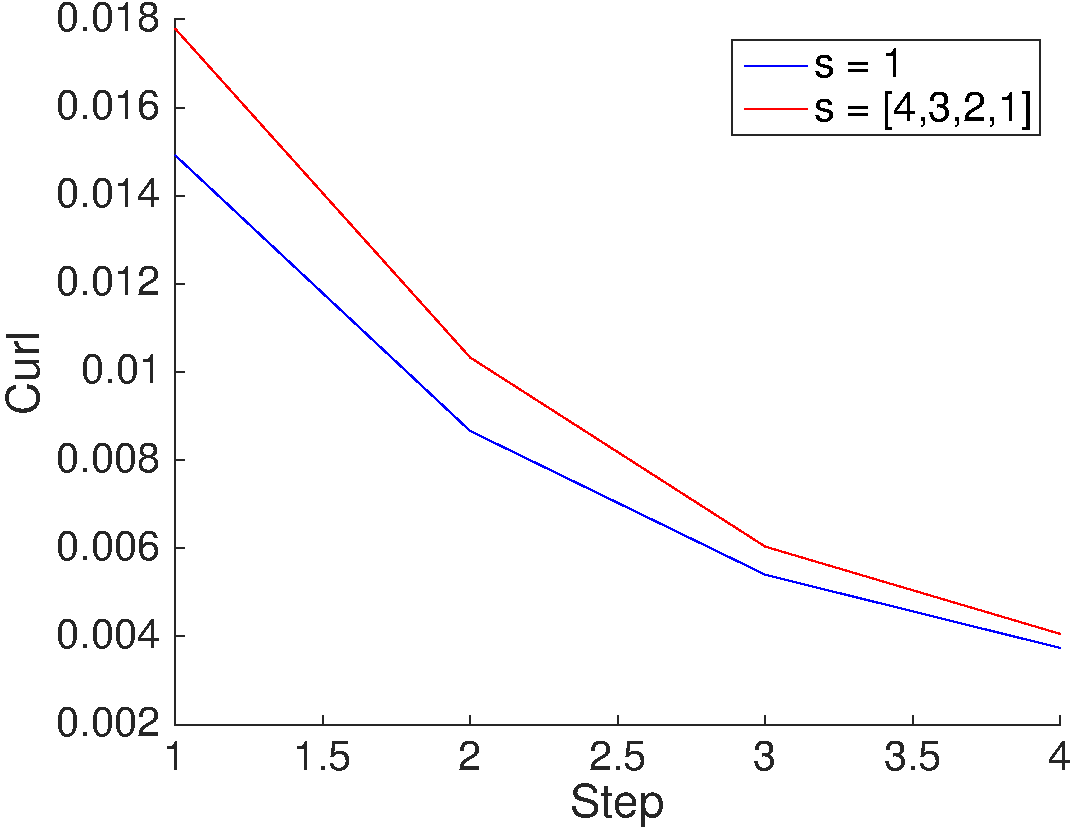
\includegraphics[width=0.55\columnwidth]{spatial_curl.pdf}}
  \subfloat[(Absolute) Divergence]{\label{subfig:spatialdiv}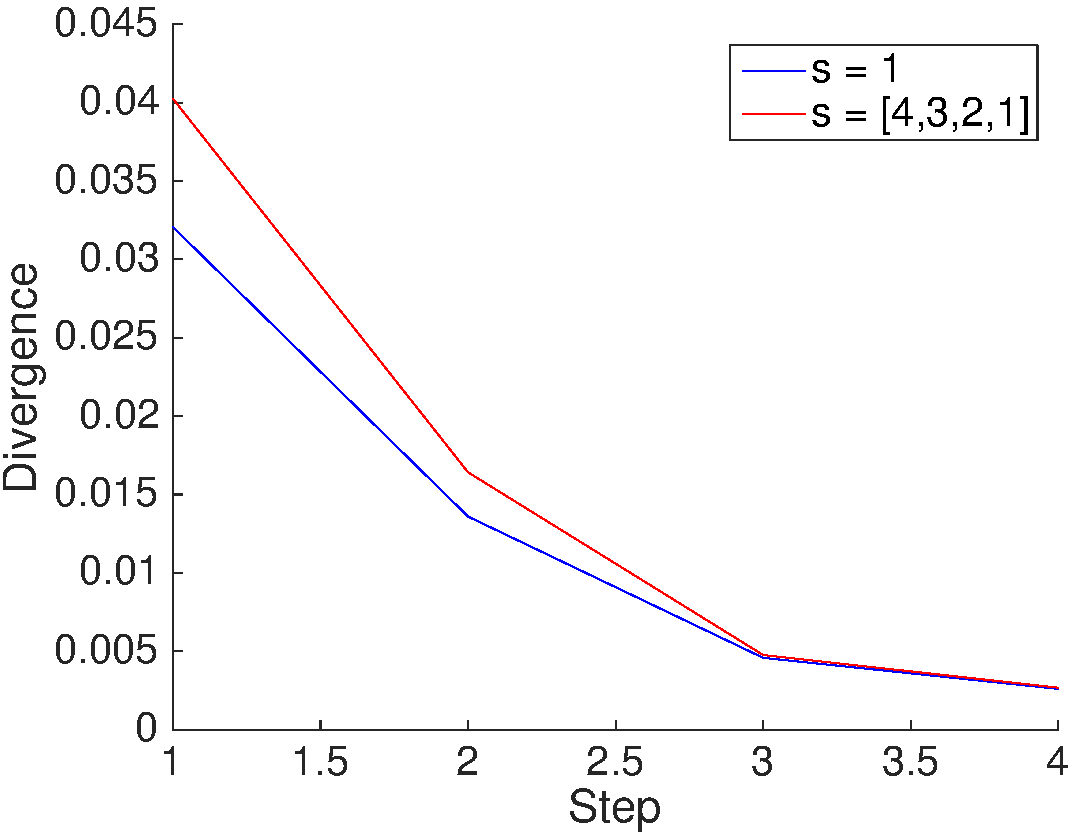
\includegraphics[width=0.55\columnwidth]{spatial_divergence.pdf}}
 % \vspace*{0.5cm} 
  \caption{Results from testing the effect of changing the spatial resolution from low to
    full. The lines are the mean over all points. For the full (blue) and low-to-full
    (red) resolution, the difference in results are (a): blue $1.42\mathrm{e}{-4}$ vs red
    $1.58\mathrm{e}{-4}$, (b): blue $3.74\mathrm{e}{-3}$ vs red $4.21\mathrm{e}{-3}$, and
    (c): blue $2.60\mathrm{e}{-3}$ vs red $2.70\mathrm{e}{-3}$.}
  \label{fig:spatialtest}
\end{figure*}
The spatial resolution is set to $s=[4,3,2,1]$, which equivalent of smoothly interpolating
every 4th point, followed by every 3rd, etc. As with the control point spacing of the
deformation field, we scale this to fit the image if the image is not equilateral. For
instance, if the image has the spatial dimension $100\times150\times50$ then space between
spatial interpolations for $s=3$ will be $[2,3,1]$ with a bound on no less than 1
(i.e. full resolution). The results are shown in \Cref{fig:spatialtest}. The results are
very similar in the final step. However, hierarchical resolution approach compared to the
full resolution gave a speedup of a factor 2.4.

\subsubsection{A Qualitative Example of the Results}
\label{subsec:qualitativeresult}

Finally, we visualize the registration to perform a qualitative assessment of the warp,
shape and orientation of the individual ODFs. All registrations are based on the raw,
noise-corrected HARDI data, while we show the tomographic inversion (FRT) indicating the
direction of the diffusion and likely fiber tract orientations. Unlike the simulated
experiments, we have fitted a B-spline to the image prior to deforming and visualizing the
result, in contrast to the smoothing spline used in the artificial examples. The results
where obtained using an increasing control point resolution with $\kappa=15$, bins
$=[50,100,200,500]$, and spatial resolution $=[4,3,2,1]$ and \Cref{fig:cc_slice_2D_result}
shows the result for the central ROI slice, along with a zoomed in version in
\Cref{fig:cc_slice_result_zoom}.

\begin{figure*}[!htb]
  \centering \subfloat[Ground
  truth]{\label{subfig:cc_slice_2D}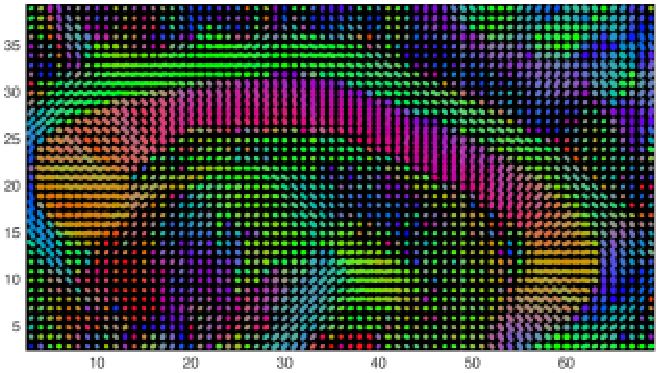
\includegraphics[width=0.6\columnwidth]{CC_slice_orig2D.pdf}}
  \subfloat[Warped
  image]{\label{subfig:cc_warp_2D}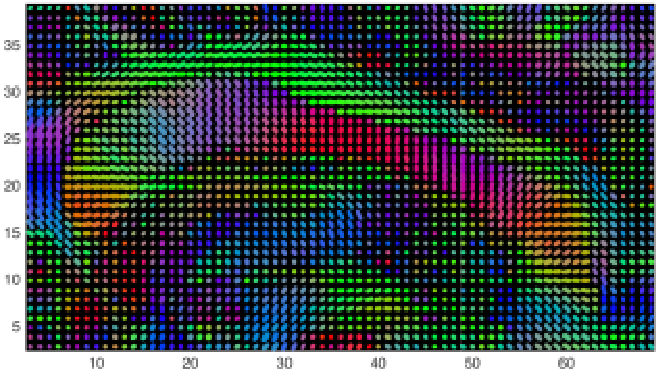
\includegraphics[width=0.6\columnwidth]{CC_slice_deform2D.pdf}}
  \subfloat[Registered image
  reconstruction]{\label{subfig:cc_warp_2D_registered}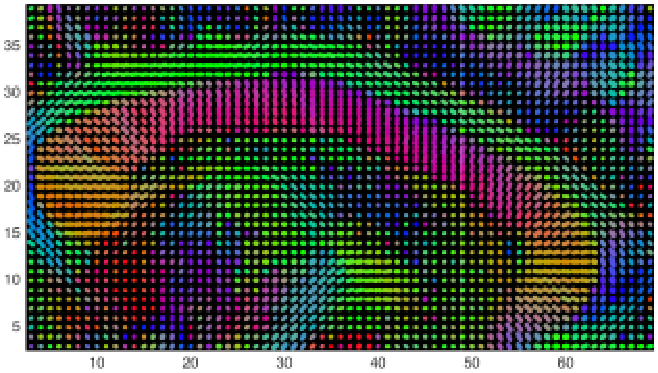
\includegraphics[width=0.6\columnwidth]{CC_slice_deform2D_best.pdf}}
  \caption{2D visualization of \Cref{subfig:cc_slice}, and the reconstructed warped image
    after applying the deformation field to the original image. We will be registering (b)
    back to (a).}
  \label{fig:cc_slice_2D_result}
\end{figure*}

\begin{figure}[!t]
  \centering
  \subfloat[Ground truth]{\label{subfig:cc_slice_3D_zoom}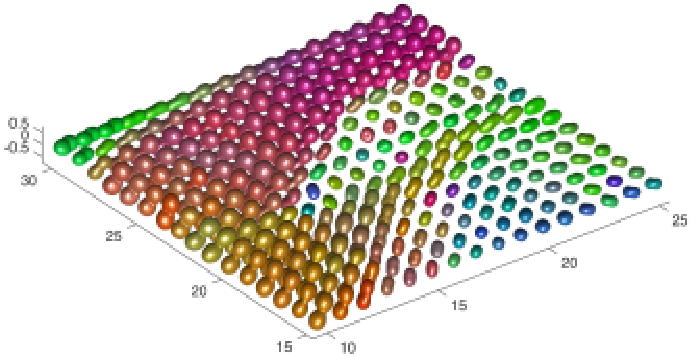
\includegraphics[width=0.9\columnwidth]{CC_slice_orig3D_zoom.pdf}}  \\
  \subfloat[Registered image
  reconstruction]{\label{subfig:cc_warp_3D_zoom_result}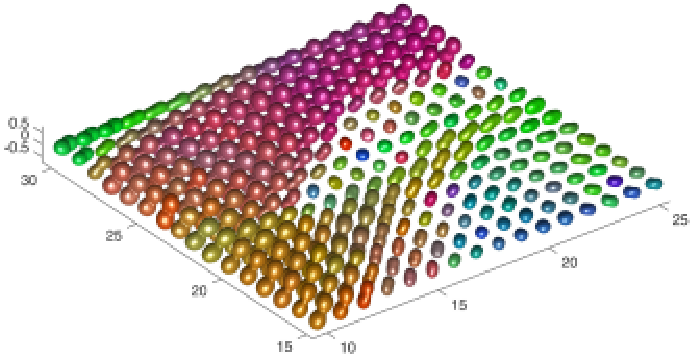
\includegraphics[width=0.9\columnwidth]{CC_slice_deform3D_zoom.pdf}}
  \caption{Same as \Cref{fig:cc_slice_2D_result}, zoomed in on the left side (anterior) of
    the figure (around the Genu). The images are not a 100 percent the same, but the
    difference is hard to notice, and the registration more than adequate.}
  \label{fig:cc_slice_result_zoom}
\end{figure}




\section{Conclusion}

We have presented a scale-space formulation of density estimation that extends LOR to
spatio-directional data, explicitly for the registration of DWI data with explicit
reorientation of the full diffusion profile. We have provided empirical evidence showing
that the underlying structure of the data is preserved during registration, while
providing excellent registration results through a number of classical artificial examples
known to be difficult for registration. In addition, we have shown that the formulation of
the similarity itself provides regularization through the additional information given by
the orientational dimension, illustrated clearly in the artificial examples. We have
investigated the different scales provided by the framework and shown how the different
parameters influences the registration results. In conclusion, the LOR-DWI provides a
smooth and well-matched deformation of DWI data, and the registration results are improved
by the induced regularization obtained by integrating the orientational information in the
objective function. Finally, we showed that the deformation have very little impact on the
shape of the deformed ODF.

\section*{Acknowledgments}
This research was supported by Centre for Stochastic Geometry and 
Advanced Bioimaging, funded by grant 8721 from the Villum Foundation.


\bibliographystyle{spmpsci}
\bibliography{IEEEabrv,mybib}
\vspace{-1cm}

% \begin{IEEEbiography}
%   [{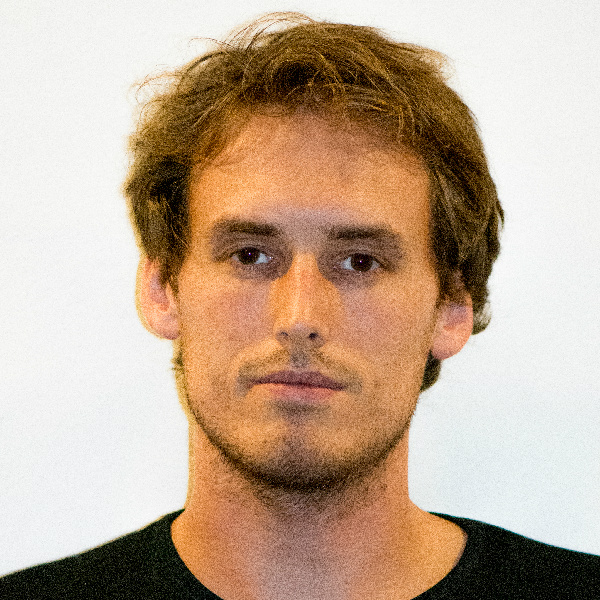
\includegraphics[width=1in,height=1.25in,clip,keepaspectratio]{croppedHenrik}}]
%   {Henrik G. Jensen} received his Masters Degree in Computer Science from the University
%   of Copenhagen in 2014. Shortly after, he was awarded an open grant and started as a PhD
%   fellow in the same department, studying medical image analysis and registration of
%   diffusion-weighted MRI. His research interests also include machine learning and data
%   analysis, and before finishing his Bachelor's Degree, he had already defended his first
%   international conference paper on automatic diagnosis of rare diseases. He has also
%   worked as a research assistant analyzing aerial drone footage with the purpose of
%   automatic weed detection to reduce the use of agricultural herbicides.
% \end{IEEEbiography}
% \begin{IEEEbiography}[{\includegraphics[width=1in,height=1.25in,clip,keepaspectratio]{francois}}]
%   {Francois Lauze} studied Mathematics in France, University of Nice Sophia Antipolis
%   where received a PhD in Algebraic Geometry in 1994. He spent some years in Burkina Faso,
%   where he taught Mathematics at the University of Ouagadougou. He moved
%   to Denmark and engaged in PhD n$^o$2, at the IT University of Copenhagen, which he
%   received in 2004. He worked on Variational Methods for Motion Compensated Inpainting and
%   motion recovery among other.He currently holds a position as Associate Professor in
%   Mathematical Image Analysis at the department of Computer Science, University of
%   Copenhagen. He has mainly worked with variational methods, and geometry for Image
%   Analysis - mainly Riemannian but also some metric geometry. More recently with inverse
%   problems in photometric stereo and tomographic imaging.
% \end{IEEEbiography}
% \begin{IEEEbiography}
%   [{\includegraphics[width=1in,height=1.25in,clip,keepaspectratio]{sune}}] {Sune Darkner}
%   received his Masters Degree in Applied Mathematics in 2004. In collaboration with Oticon
%   A/S, he received his Industrial Ph.D. degree in Shape and Deformation Analysis of the
%   Human Ear Canal in 2009, from the Department of Informatics and Mathematical Modelling,
%   at the Technical University of Denmark (DTU). After holding a position at an energy
%   company as data analyst, he rejoined the Department of Informatics and Mathematical
%   Modelling at DTU in 2009 as a post doc. He currently holds a position as Associate
%   Professor in image analysis at the Department of Computer Science, University of
%   Copenhagen. Research interests include image registration and classification,
%   optimization and regularization, and computational physics.
% \end{IEEEbiography}
% %

\end{document}


